\documentclass[12pt, british]{ntnuthesis} 
\addbibresource{thesis.bib}

% From https://www.overleaf.com/learn/latex/Glossaries

\makeglossaries % Prepare for adding glossary entries



% --------------------
% ----- Acronyms -----
% --------------------

\newacronym[type=\acronymtype]{CP}{CP}{Cerebral Palsy}

\newacronym[type=\acronymtype]{CNN}{CNN}{Convolutional Neural Network}

\newacronym[type=\acronymtype]{GCN}{GCN}{Graph Convolutional Network}

\newacronym[type=\acronymtype]{GNN}{GNN}{Graph Neural Network}

\newacronym[type=\acronymtype]{HAR}{HAR}{Human Action Recognition}

\newacronym[type=\acronymtype]{NTNU}{NTNU}{Norwegian University of Science and Technology}

\newacronym[type=\acronymtype]{ANN}{ANN}{Artificial Neural Network}

\newacronym[type=\acronymtype]{NAS}{NAS}{Neural Architecture Search}

\newacronym[type=\acronymtype]{AutoML}{AutoML}{Automated Machine Learning}

\newacronym[type=\acronymtype]{GPU}{GPU}{Graphics Processing Unit}

\newacronym[type=\acronymtype]{DAG}{DAG}{Directed Acyclic Graphs}

\newacronym[type=\acronymtype]{EC}{EC}{Evolutionary Computations}

\newacronym[type=\acronymtype]{BO}{BO}{Bayesian Optimisation}

\newacronym[type=\acronymtype]{EcoNAS}{EcoNAS}{Economical Evolutionary-based NAS}

\newacronym[type=\acronymtype]{AGNN}{AGNN}{Automated Graph Neural Networks}

\newacronym[type=\acronymtype]{SNIP}{Snip}{Single-shot Network Pruning}

\newacronym[type=\acronymtype]{GRASP}{Grasp}{Gradient Signal Preservation}

\newacronym[type=\acronymtype]{Synflow}{Synflow}{Iterative Synaptic Flow Pruning}

\newacronym[type=\acronymtype]{AUC}{AUC}{Area Under the receiver operating characteristic Curve}

\newacronym[type=\acronymtype]{Auto-GNN}{Auto-GNN}{Automated Graph Neural Network}

\newacronym[type=\acronymtype]{FLOPs}{Flops}{Floating Point Operations per second}

\newacronym[type=\acronymtype]{VCNN}{VCNN}{Vanilla Convolutional Neural Network}

\newacronym{ntu-rgbd}{NTU RGB+D}{Nanyang Technological University's Red Blue Green and Depth-information}


  % add glossary and acronym lists before document
\begin{document}
%\begin{titlepage}
        \vspace*{0.3cm}
        \noindent
        \textcolor{gray}{\Large Zaim ul-Abrar Imran}\\[0.2cm]
        \textcolor{gray}{\Large Max Torre Schau}\\
        
        \vspace{0.6cm}
        \begin{comment}
            
        { \noindent \huge \bfseries Investigating Zero-Cost proxies on Graph Convolutional Networks on Human Action Recognition-tasks}
        \end{comment}
        
        {\noindent \LARGE \bfseries Exploring the Efficiency of Zero-Cost Proxies in NAS for Human Action Recognition }\\


        \vspace{6.0cm}
        \noindent
        Computer Science, Master's Thesis \\
        Supervisor: Heri Ramampiaro\\
        Co-supervisor: Espen A. F. Ihlen \& Felix Tempel\\     
        June 2023\\

        \vspace{0.8cm} 
        \noindent
        Norwegian University of Science and Technology\\
        Faculty of Information Technology and Electrical Engineering\\
        Department of Computer Science\\
       
        \vspace{0.8cm}
        \noindent
        \includegraphics[width=0.40\textwidth]{figures/NTNU_logo.png}
\end{titlepage}

\chapter*{Abstract}

In the rapidly evolving field of Graph Convolutional Networks (GCNs), the architecture selection process through Neural Architecture Search (NAS) remains a crucial yet challenging task. The core focus of this thesis is to investigate the application and performance of zero-cost proxies for evaluating GCNs within the context of Human Activity Recognition (HAR) tasks as a first step towards using them in a NAS algorithm. Furthermore, given the need for more research, the study aims to bridge this gap by evaluating different zero-cost proxies on GCN architectures. 

To the best of our knowledge, the study is the first in the literature to exhibit how zero-cost proxies perform on GCNs. In addition, the authors did a quantitative study on how zero-cost proxies perform by creating an extensive benchmark of trained architectures for HAR tasks.

Through a series of analyses and experiments, the study demonstrated that integrating zero-cost proxies can significantly enhance the efficiency and accuracy of NAS algorithms. The results revealed that the top-performing zero-cost proxies displayed a Spearman $\rho$ of approximately $0.8$, indicating a very strong correlation. However, no substantial improvement in correlation was detected when analysing architectures as they were trained for several epochs, implying that the zero-cost proxies might be most efficient at the initialisation of the neural network. Attempts to combine zero-cost proxies using vote and weighted arithmetic mean showed potential but did not yield considerable improvement compared to the individual application of each zero-cost proxy. 
\chapter*{Sammendrag}

I det raskt utviklende feltet Graph Convolutional Networks (GCNs), er arkitekturvalgprosessen gjennom Neural Architecture Search (NAS) fortsatt en avgjørende, men utfordrende oppgave. Hovedfokuset i denne avhandlingen er å undersøke anvendelsen og ytelsen til zero-cost proxies for evaluering av GCNs innenfor oppgaver for gjenkjennelse av menneskelig aktivitet (HAR). Basert på behovet for mer forskning i feltet, tar studien sikte på å bygge bro over dette gapet ved å evaluere forskjellige zero-cost proxies på GCN-arkitekturer. 

Så vidt vi vet, er studien den første i litteraturen til å vise hvordan zero-cost proxies presterer på GCNs. Forfatterne gjorde en kvantitativ studie på hvordan zero-cost proxies presterer ved å lage en omfattende benchmark av trente arkitekturer for HAR-oppgaver. 

Gjennom en serie analyser og eksperimenter, viste studien at integrering av zero-cost proxies kan øke effektiviteten og nøyaktigheten til NAS-algoritmer betydelig. Resultatene viser at de zero-cost proxiesene som presterer best viste en Spearman $\rho$ på omtrent $0.8$, noe som indikerer en veldig sterk korrelasjon. Imidlertid ble ingen betydelig forbedring i korrelasjon oppdaget når arkitekturene ble analysert etter å ha blitt trent i flere epoker, noe som antyder at zero-cost proxies er mest effektive ved initialiseringen av det nevrale nettverket. Forsøk på å kombinere zero-cost proxies ved hjelp av stemmegiving og vektet aritmetisk gjennomsnitt viste potensial, men ga ikke noen betydelig forbedring sammenlignet med å bruke zero-cost proxies individuelt. 
\chapter*{Preface}
This is the final project for our Master's in Computer Science at the Norwegian University of Science and Technology (NTNU). It's written by us, Zaim ul-Abrar Imran and Max Torre Schau, and is the last step in our studies. 

The project is part of DeepInMotion, a collaboration project between NTNU and St. Olavs Hospital in Trondheim. Head of Department and Professor at the Department of Computer Science, Heri Ramampiaro has been the main supervisor of this Master's thesis, with Associate Professor at the Department of Neuromedicine and Movement Science, Espen Alexander F. Ihlen and  PhD Candidate at the Department of Computer Science, Felix Tempel as co-supervisors. 
\chapter*{Acknowledgement}
We would first like to thank our supervisor, Heri Ramampiaro, for allowing us to work on the project. His guidance, support, and encouraging feedback have been invaluable. He also gave us many chances to showcase and discuss our work, which we found both inspiring and educational.

We would also like to thank our co-supervisors, Associate Professor Espen Alexander F. Ihlen and PhD Candidate Felix Tempel. Their expert advice and continuous support have been instrumental in our project's success. In addition, they provided us with constructive critiques and guidance that significantly improved our work. We are deeply grateful for their invaluable contribution to our learning experience.

Lastly, we want to thank our friends. Your friendship, helpful advice, and all the fun times we have had together truly helped us through our time at NTNU. We are so grateful for your support during this part of our lives.

\begin{flushright}
\textit{To Zaim: Thank you for being a fellow student, colleague, collaborator, problem-solver, and, most importantly, a best friend through my five years at NTNU.} \\
- Max
\end{flushright}

\begin{flushright}
\textit{To Max: The past five years have been an incredible journey of friendship and partnership. Our shared experiences, from late-night study sessions to exhilarating concerts, from challenging school projects to roaring cheers on the football field, our bond has grown deeper and stronger with every shared experience. Your support and friendship have been invaluable; I am deeply grateful. Thank you, my friend, for being a part of my life, and I look forward to the adventures yet to come.} \\
- Zaim
\end{flushright}




\tableofcontents
\listoffigures
\listoftables
\listofalgorithms
\renewcommand{\glsnamefont}[1]{\textbf{#1}}
\printglossary[type=\acronymtype,nonumberlist,style=super,nogroupskip] % Print acronyms
\chapter{Introduction}
\begin{comment}
This chapter will introduce the thesis by stating its background and motivation. In addition, we will specify the main goal and the research questions. Lastly, we will present what contributions the thesis makes in addition to the overall structure of the thesis. 
\end{comment}
Chapter 1 of this thesis introduces the background and motivation behind the research, as well as the problem statement and scope of the study. It also includes the main goal and research questions, which aim to investigate the potential of using zero-cost proxies to enhance the efficiency and accuracy in \Gls{NAS} algorithms, specifically for \Gls{GCN} applied to \Gls{HAR} tasks. Finally, the chapter concludes with a section on the research method and contributions of the study.

 \section{Background and Motivation}
This thesis is written as part of a project named DeepInMotion. Researchers from the \Gls{NTNU} and St. Olavs Hospital cooperate in a cross-disciplinary collaboration involving child physiotherapists, paediatricians, neonatologists, movement scientists and computer engineers. The project has developed a pipeline for detecting \Gls{CP} in infants by providing a video of the infant's movement. The pipeline employs a \Gls{CNN} to accurately extract movement from 2D images or videos \autocite{groos2021efficientpose}. A \gls{GCN} then processes the output to predict \gls{CP} in high-risk infants at three months of age \autocite{groos2022convolutional}. 

The \gls{CP}-prediction pipeline used \gls{NAS} to automatically find a suitable architecture which yields good results in regards to the performance of the model. However, the search could be faster and more efficient while providing good results. Performance predictor is a way of estimating the relative performance of an architecture for a given problem and can be far more effective than training the architecture until convergent. There needs to be more research on using zero-cost proxies with \gls{GCN}. This gap in the literature means that potential improvements in the efficiency and performance of \gls{NAS} when using \gls{GCN} might still need to be discovered. The \gls{CP}-prediction pipeline could be enhanced by addressing this gap, and additional knowledge about how zero-cost proxies can be used with graph-based learning could be gained. This research aims to explore the effectiveness of zero-cost proxies in conjunction with \gls{GCN} and uncover how they perform. 
\section{Problem Statement}\label{ProblemStatement}
In recent years, NAS has emerged as a promising technique for automating designing neural networks with excellent performance on specific tasks \autocite{zoph2016neural}. Several studies have shown that NAS can effectively identify suitable architectures for GCN problems, widely used in social network analysis, bioinformatics applications and human action recognition. However, despite the recent advancements in NAS for GCN, evaluating architectures in existing studies remains a significant challenge. It is often infeasible to thoroughly train each candidate's architecture to obtain its ground truth accuracy \autocite{zoph2016neural}. This issue is particularly pressing in resource-constrained environments, where training large numbers of models is infeasible.

Moreover, a significant limitation of the existing literature on GCN-NAS is the absence of performance predictors, further complicating the optimisation process. The lack of such predictors can make it challenging to identify the most promising architectures for a given task efficiently. Evaluating every architecture can be prohibitively time-consuming and computationally expensive. Novel approaches, such as zero-cost proxies, have been proposed to predict candidate architectures' performance without requiring full training. However, there is still much work to be done in exploring the efficacy of these approaches and optimising them for GCN-NAS.
\section{Scope of the Thesis}

This thesis investigates the potential of utilising zero-cost proxies to enhance the efficiency and accuracy of architecture search in NAS algorithms, specifically targeting GCN applied to HAR tasks. The research questions formulated for this study are designed to explore various aspects of zero-cost proxies and their effectiveness in ranking GCN architectures.

Nonetheless, it is crucial to outline the scope and limitations of this thesis to ensure that readers understand which topics will and will not be discussed in detail. Although the overall goal is to improve and optimise the efficiency of NAS with GCN for HAR, the primary focus of this study is to analyse and evaluate different zero-cost proxies and their combinations. As a result, a full implementation of the research findings within an actual NAS algorithm will not be provided.

By clarifying the scope of this thesis, the intention is to offer readers a more comprehensive understanding of the research focus and the study's limitations. While recognising that incorporating the findings into a practical NAS algorithm constitutes an essential and valuable subsequent step, the primary objective of this thesis is to lay the foundation for future research by exploring the potential of zero-cost proxies in the context of GCN for HAR tasks.
\begin{comment}
\textbf{Research Question 2} \textit{How does the relationship between zero-cost proxies and validation accuracy evolve during the warm-up phase of GCN training, and how early can we potentially halt the training process?}
\end{comment}
\begin{comment}
\textbf{Research Question 2} \textit{How does the correlation between zero-cost proxies and validation accuracy change during the warm-up phase, as GCN architectures are trained for up to 10 epochs? }

This research question investigates the relationship between zero-cost proxies and validation accuracy during the initial training phase (referred to as the warm-up phase) of GCN architectures. Specifically, it seeks to understand how the predictive power of zero-cost proxies evolves as architectures are trained for up to 10 epochs. 
\end{comment}

\begin{comment}
\textbf{Research question 3}\textit{ How will combining zero-cost proxies improve neural architecture search for GCN?}

Studies on zero-cost proxies on different computer vision tasks using CNN show that combining them may yield better performance than using them independently. Therefore, we will investigate how we can use an ensemble of zero-cost proxies in a neural architecture search for GCN. 


\textbf{Research question X} \textit{How can we effectively combine zero-cost proxies using various techniques, such as supervised learning, feature engineering, and weighted averaging, to enhance the efficiency and accuracy of architecture search in Neural Architecture Search (NAS) algorithms?}
\end{comment}
\section{Goal and Research Questions}\label{section:goalsandrq}

\textbf{Goal} \textit{Improve and optimise the efficiency of neural architecture search with graph convolutional networks for human action recognition.} 

NAS has been used with GCN in different studies \autocite{zhou2019auto, groos2022toward, peng2020learning}, but finding other, more efficient methods is still possible. If one can find ways far more effective than what exists today, more architectures can be researched, which may result in detecting other well-performing architectures. Also, as training and searching for neural networks may impact the environment, effective methods will significantly reduce the carbon footprint. 

\textbf{Research question 1} \textit{How well can different zero-cost proxies rank GCN architectures compare to their validation accuracy?}

Recent studies \autocite{abdelfattah2021zero, colin2022adeeperlook} show that zero-cost proxies yield great promise regarding using it to rank different architectures. However, to the authors´ knowledge, research is yet to be done on how zero-cost proxies perform on GCN architectures. Evaluating the correlation between zero-cost proxies and ground truth validation accuracy can determine if they accurately indicate the ground truth.


\textbf{Research Question 2} \textit{How early can we identify the correlation between zero-cost proxies and validation accuracy during the warm-up phase of GCN training to potentially halt the training process sooner?}


Research Question 2 aims to investigate the potential for early identification of the correlation between zero-cost proxies and validation accuracy during the warm-up phase of training for GCN. In addition, this research question aims to determine if it is possible to score network before fully training it. 


\textbf{Research question 3} \textit{How can we effectively combine zero-cost proxies using various techniques to enhance the efficiency and accuracy of architecture search in NAS algorithms?}

Through investigating Research Question 3, the study aims to identify effective techniques for combining zero-cost proxies to enhance the efficiency and accuracy of architecture search. By leveraging the strengths of multiple zero-cost proxies, future NAS algorithms may become more efficient and accurate in discovering high-performing architectures. The outcomes of this research question can provide insights into how to optimise the use of zero-cost proxies in NAS algorithms and improve the architecture search process in the future.

\begin{comment}
While theory and analysis can be used for heuristics and rationale when designing models,
modern deep learning is commonly researched through experiments where multiple
alternatives are compared based on relevant metrics.
This thesis employs an experimental research method to study the problem area and
answer the research questions. Generated models from the project experiments are
compared based on pre-specified evaluation criteria on dedicated training and validation
sets to advance the models iteratively. Lastly, the final models are compared and evaluated
on an unseen test set.
\end{comment}

\begin{comment}
    This project is based on a quantitative study where alternative solutions are eval-
uated based on their statistical performance on the relevant problem. Initially,relevant approaches are assessed to gather information about the state-of-the-art methods related to the problem. Based on the analysis of these methods, we hy-
pothesize what can be improved with the given methods and use this as a guideline when proposing our method. Appropriate evaluation metrics are selected before evaluating the proposed method and comparing it with the state-of-the-art approaches, and a dataset on which experiments are performed is acquired. Subsequently, experiments are carried out, and comparisons of the different methods can be obtained. Accordingly, observations and conclusions are extracted from the
experiments.
\end{comment}
\section{Research Method}
The researchers conducted a comprehensive literature review in the fall of 2022 to understand current state-of-the-art approaches in the field of \gls{NAS}. In addition, a systematic review of relevant studies focused on performance predictors within the \gls{NAS} domain was also carried out. The project's conclusion presents several recommendations for advancing research in the \gls{NAS} field based on the insights gained from the review.

The research plan involves conducting multiple quantitative investigations to examine the performance and behaviour of zero-cost proxies on a \gls{HAR} dataset. Subsequently, the study aims to explore the potential of these proxies in improving \gls{NAS} processes.



\section{Contributions}

This thesis presents several critical contributions to the \gls{NAS} field with \glspl{GCN} for \gls{HAR}. The following are the primary contributions made by this study:

\textbf{Investigation of Zero-Cost Proxies:} In this thesis, a thorough analysis of the relationship between zero-cost proxies and the performance of \gls{GCN} models in \gls{HAR} tasks is conducted. The study sheds light on the usefulness of using zero-cost proxies to estimate the performance of \gls{GCN} architectures without the need for costly training. To our knowledge, this research is the first in the literature to specifically explore the application of zero-cost proxies within the context of \gls{GCN} tasks.

\textbf{Combining Zero-Cost Proxies:} The thesis presents effective methods, such as the majority vote method and the weighted arithmetic mean method, for combining different zero-cost proxies to improve the efficiency and accuracy of the \gls{NAS} process. 

\textbf{Environmental Considerations:} The study highlights the importance of considering the environmental implications of \gls{NAS} and artificial intelligence research. Furthermore, the study contributes to developing more sustainable practices in the field by reducing the \gls{NAS} process's computational demands and training time.

In view of these contributions, the work in this thesis advances the understanding of \gls{NAS} with \glspl{GCN} in the context of \gls{HAR} and provide a foundation for further exploration of zero-cost proxies and their potential applications.
\section{Thesis outline}

The thesis consists of the following seven chapters:

\textbf{Chapter 1 - Introduction:} The introductory chapter presents the study's background, motivation, problem statement, scope, goal, and research questions.

\textbf{Chapter 2 - Theory:} Chapter 2 introduces necessary background theory, including deep learning, \gls{NAS}, \gls{GCN} and \gls{HAR}.  

\textbf{Chapter 3 - Related Work:} A comprehensive review of the literature on \gls{NAS} and \gls{GCN}-\gls{NAS} is provided, encompassing zero-cost proxies and recent research on \gls{GCN}-\gls{NAS}. In addition, a discussion on the gap and limitations in the literature is presented. 

\textbf{Chapter 4 - Method:} This chapter covers the use of zero-cost proxies in \gls{NAS}, including various proxies and their implementation, the use of warmup, and the combination of proxies using a custom vote measure and weighted arithmetic mean. 

\textbf{Chapter 5 - Results:} The results, namely the correlation analysis, vote measure and weighted arithmetic mean, are presented in this chapter. 

\textbf{Chapter 6 - Discussion:} This chapter discusses the study's findings and analyses and interprets the results and their implications. In addition, it discusses the study's limitations as well as the environmental implications.

\textbf{Chapter 7 - Conclusion and Future Work:} The conclusion of the thesis summarises the findings and discusses future work. 

\chapter{Theory}
\begin{comment}
This chapter will contain the essential theory for the thesis. 

As the authors did a literature review as a pre-study for this project, some subchapters will be re-used as the theory is still highly relevant for this thesis. 
\end{comment}
Chapter 2 of the thesis introduces the challenges of using machine learning with graphs and how \glspl{GCN} have emerged as a solution to these challenges. The chapter describes the core of \glspl{GCN}, the graph convolution operation, and how it aggregates local information from neighbouring nodes to generate a new representation for each node. The chapter also introduces \Gls{AutoML}, an emerging area of machine learning that seeks to automate designing optimal machine learning architectures. Finally, the chapter provides an overview of \gls{NAS}, a sub-field of \gls{AutoML} that aims to automate creating of high-performing neural networks and \gls{HAR}. 

\section{Deep Learning} 
Deep learning, a subfield of machine learning, has gained significant attention in recent years due to its ability to learn hierarchical representations from raw data, especially in domains such as computer vision, natural language processing, and speech recognition. This contrasts conventional machine-learning techniques, which are limited in processing the same \autocite{lecun2015deep}. 

The core building blocks of deep learning are \Gls{ANN} inspired by the biological neural networks found in the human brain. ANNs consist of interconnected layers of artificial neurons called nodes, with each node receiving input from previous layers, processing the information, and propagating the output to the subsequent layers. Deep learning architectures typically involve multiple layers of these interconnected nodes, hence the term "deep" \autocite{goodfellow2016deep}.

One key advantage of deep learning over traditional machine learning techniques is its ability to automatically learn and extract features from raw data without relying on manual feature engineering. This process, called representation learning, enables deep learning models to understand hierarchical representations of the input data, with each layer capturing increasingly abstract and complex features \autocite{bengio2013representation}. This capability has led to breakthrough performance improvements in various applications, including image classification, natural language understanding, and speech recognition \autocite{krizhevsky2017imagenet}.
\subsection{Neural Networks}\label{neuralnet}
Neural Networks are a part of neurocomputing, a field of study that aims to develop computational systems inspired by the human brain's structure and function. For example, pattern recognition, motor control, vision, flexible inference, intuition, and accurate guessing are all skills the brain is particularly adept at, which is what neural networks aim to emulate \autocite{anderson1995introduction}. 

At a high level, a neural network is a collection of interconnected nodes (called "neurons") arranged in layers. The input layer receives input data, which is passed through one or more hidden layers before the output from the final layer.

The basic unit of a neural network is a neuron, which receives input from other neurons or the input layer. The neuron then applies a mathematical function to this input, producing an output sent to other neurons in the next layer. The most commonly used function is the sigmoid function, given in \cref{eq:sigmoid}. 

\begin{equation}
    \sigma(z) = \frac{1}{1+e^{-z}}
    \label{eq:sigmoid}
\end{equation}

where $z$ is the input to the neuron, the sigmoid function has the valuable property that its output is always between 0 and 1, which can be interpreted as a probability.

The output of a neuron is determined by the weights and biases associated with its inputs. Each input is multiplied by a weight, and these weighted inputs are summed together with a bias term to produce the neuron's input, as shown in \cref{eq:z}. 

\begin{equation}
    z = \sum_{i=1}^n w_i x_i + b
    \label{eq:z}
\end{equation}

where $w_i$ is the weight associated with the $i$th input, $x_i$ is the value of the $i$th input, $n$ is the number of inputs, and $b$ is the bias term.

\Cref{eq:y} exhibits the neuron output when applying the sigmoid function to the input.

\begin{equation}
    y = \sigma(z)
    \label{eq:y}
\end{equation}

During the training process, which comprises feeding training data through the network (illustrated in \cref{fig:nn}) and modifying the weights and biases based on the difference between the predicted output and the actual output, the weights and biases of a neural network are changed. Usually, a gradient descent optimisation technique is used to carry out this operation.

\begin{figure}[h]
\resizebox{\textwidth}{!}{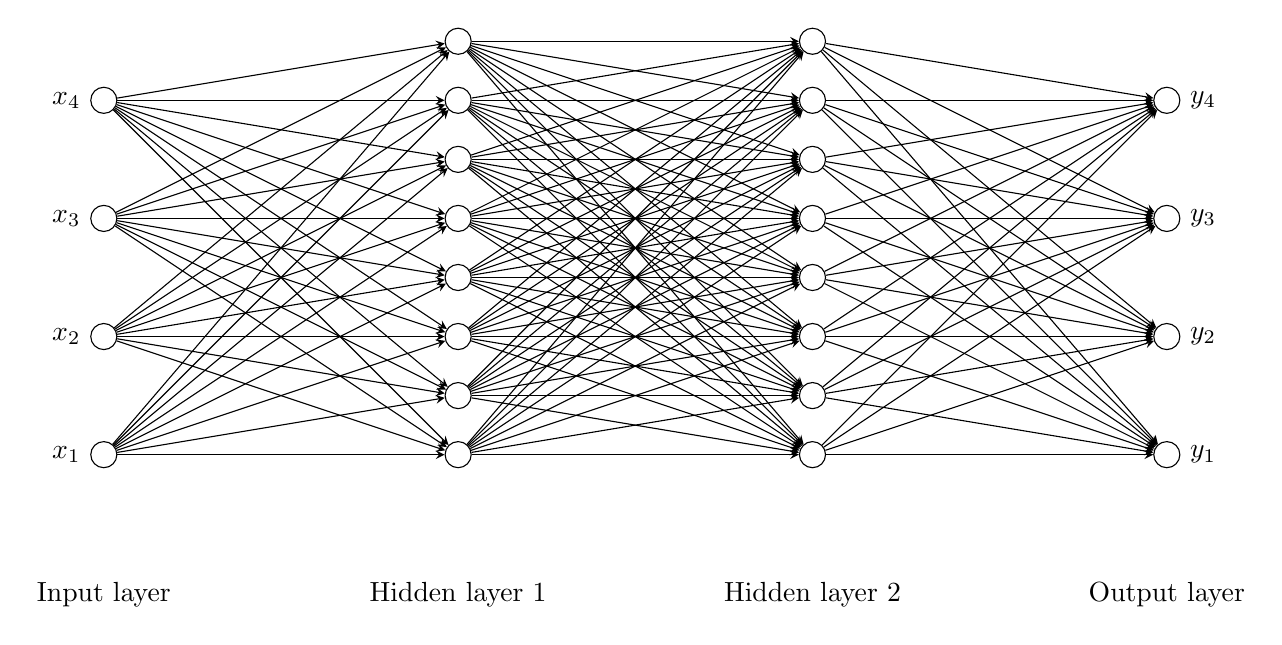
\begin{tikzpicture}[x=3cm, y=1.5cm, >=stealth]
    
    % Input layer nodes
    \foreach \i in {1,...,4} {
        \node[draw, circle] (input-\i) at (0, \i) {};
    }
    
    % First hidden layer nodes
    \foreach \i in {1,...,8} {
        \node[draw, circle] (hidden1-\i) at (1.5, 0.5 + 0.5*\i) {};
    }
    
    % Second hidden layer nodes
    \foreach \i in {1,...,8} {
        \node[draw, circle] (hidden2-\i) at (3, 0.5 + 0.5*\i) {};
    }
    
    % Output nodes
    \foreach \i in {1,...,4} {
        \node[draw, circle] (output-\i) at (4.5, \i) {};
    }

    % Input layer labels
    \foreach \i in {1,...,4} {
        \node[left] at (input-\i.west) {$x_{\i}$};
    }
    
    % Output layer labels
    \foreach \i in {1,...,4} {
        \node[right] at (output-\i.east) {$y_{\i}$};
    }
    
    % Connect input to first hidden layer
    \foreach \i in {1,...,4} {
        \foreach \j in {1,...,8} {
            \draw[->] (input-\i) -- (hidden1-\j);
        }
    }
    
    % Connect first hidden layer to second hidden layer
    \foreach \i in {1,...,8} {
        \foreach \j in {1,...,8} {
            \draw[->] (hidden1-\i) -- (hidden2-\j);
        }
    }
    
    % Connect second hidden layer to output
    \foreach \i in {1,...,8} {
        \foreach \j in {1,...,4} {
            \draw[->] (hidden2-\i) -- (output-\j);
        }
    }
    
    % Layer labels
    \node[below] at (0, 0) {Input layer};
    \node[below] at (1.5, 0) {Hidden layer 1};
    \node[below] at (3, 0) {Hidden layer 2};
    \node[below] at (4.5, 0) {Output layer};

\end{tikzpicture}}
\caption{Illustration of Neural Network}
\label{fig:nn}
\end{figure}

\section{Graph Convolutional Networks}

Graphs are ubiquitous structures representing complex systems, including social networks, biological networks, and transportation systems \autocite{scarselli2008graph}. They consist of nodes and edges, representing the many entities and relationships between them. Despite their widespread use, graphs pose unique challenges in machine learning due to their irregular structure, which makes it difficult to apply conventional learning techniques that rely on fixed-size inputs and Euclidean data representations \autocite{battaglia2018relational}.

\Gls{GNN} has emerged as a solution to these challenges, generalising deep learning techniques to graph-structured data \autocite{gori2005new}. Among \glspl{GNN}, \glspl{GCN} have become particularly popular owing to their ability to perform localised and efficient convolutions on graph data \autocite{DBLP:journals/corr/KipfW16}. \glspl{GCN} extend the concept of convolution from grid-like structures, such as images, to irregular graph structures, enabling the extraction of meaningful features from graph data while preserving their spatial relationships \autocite{bronstein2017geometric}. 

\subsection{Graph Convolutions}
The core of \glspl{GCN} lies in the graph convolution operation, which aims to aggregate local information from neighbouring nodes to generate a new representation for each node. The main idea is to perform a weighted sum of the feature vectors of a node and its neighbours, where the weights are determined by the edge weights or some measure of node similarity. This aggregation scheme allows \glspl{GCN} to learn node representations that effectively capture the local graph structure. The \cref{eq:kiph}, found in \autocite{DBLP:journals/corr/KipfW16}, shows how the graph convolution operation are mathematically described.

\begin{equation*} 
    \bm{H}^{l+1} = \sigma(\bm{\hat{D}}^{-\frac{1}{2}} \bm{A} \bm{\hat{D}}^{-\frac{1}{2}} \bm{H}^{l} \bm{W}^{l} )
    \label{eq:kiph}
\end{equation*}


The components in \cref{eq:kiph} are defined as follows:

$H^{(l+1)}$ stands for the updated node representations (features) at layer $(l+1)$, while $H^{(l)}$ indicates the node features at layer $l$. $H^{(0)}$ is the input feature matrix for the first layer. The graph's adjacency matrix, represented by $A$, is modified to incorporate self-connections. This is achieved by adding a diagonal matrix with ones to the original adjacency matrix $A$, ensuring that the node's features are considered during the aggregation process.

The degree matrix, denoted by $\hat{D}$, corresponds to the modified adjacency matrix $\hat{A}$. It is a diagonal matrix wherein each diagonal entry signifies the degree (number of connections) of the corresponding node. The learnable weight matrix at layer $l$ is represented by $W^{(l)}$ and is employed to linearly transform the node features at each layer.

Lastly, the activation function $\sigma$ introduces non-linearity to the model. Typical choices for activation functions are ReLU, sigmoid, and tanh.





\section{AutoML}\label{section:automl}
\glsreset{AutoML}

Fields such as computer vision, speech recognition, and natural language processing have seen significant progress, primarily due to the development and application of deep learning techniques in recent years. However, despite these advancements, designing optimal machine learning architectures remains complex and time-consuming for data scientists. \Gls{AutoML} is an area that seeks to automate this process.  

\subsection{Hyperparameter Optimisation}\label{subsection:hyperparameter-optimization}
Hyperparameter optimisation is a critical component of the \gls{AutoML} pipeline. Machine learning algorithms often contain hyperparameters that control their behaviour, and their optimal values are not learned directly from the training data. Instead, these parameters need to be set manually or searched for systematically. Traditional techniques for hyperparameter tuning include grid search, random search, and manual tuning. However, these approaches can be computationally expensive and inefficient.
\gls{AutoML} aims to streamline this process by employing advanced techniques such as Bayesian optimisation, evolutionary algorithms, and gradient-based methods. These methods can efficiently explore the hyperparameter space and identify suitable configurations, ultimately leading to improved model performance and reduced computational cost \autocite{bergstra2011algorithms, snoek2012practical}.

\subsection{Meta-learning}\label{subsection:meta-learning}
Meta-learning, also called "learning to learn," is another crucial component of \gls{AutoML}. The central idea is to utilise prior knowledge gained from solving multiple related tasks to improve the learning efficiency and generalisation ability on new tasks. This is achieved by learning a model or an algorithm that can adapt quickly to novel tasks with limited data.
In the context of \gls{AutoML}, meta-learning can be employed in various ways. One popular approach is to use meta-learning for transfer learning, wherein a pre-trained model is fine-tuned on a new task with limited available data \autocite{pan2010survey}. Another application of meta-learning is hyperparameter optimisation, where a meta-model can be trained to predict the performance of different configurations across various tasks. This knowledge can guide the search for optimal hyperparameters more efficiently \autocite{swersky2014freeze}.
\section{Neural Architecture Search (NAS)} \label{section:nas}
 \glsreset{NAS}
Most neural architectures are created by specialists, which is labour-intensive and susceptible to other weaknesses, including the need for an extensive expertise and the potential to introduce human bias. Subsequently, a way of automatically designing and developing such algorithms has been a research field for a couple of years. \gls{NAS} aims to automate the previously manual process of designing architectures \autocite{elsken2019neural}. Consequently, \gls{NAS} is a sub-field of \gls{AutoML}. 

Given a search space $F$, a training set $D_{\text{train}}$, validation set $D_{\text{valid}}$ and an evaluation metric $M$, a \gls{NAS} algorithm aims at finding an optimal architecture $f^* \in F$ with the best metric $M^*$ (such as validation accuracy) on the validation set $D_{\text{valid}}$. This can be written mathematically as shown in \cref{eq:nas}

\begin{equation}\label{eq:nas}
\begin{aligned}
    f^* &= \text{argmax}_{f \in F} M(f(\theta^*), D_{\text{valid}}), \\
    \theta^* &= \text{argmin}_{\theta} L(f(\theta), D_{\text{train}}),
\end{aligned}
\end{equation}

where $\theta^*$ is the learned parameters for the architecture $f$ and $L$ is the loss function \autocite{zhou2019auto}. 

\Cref{fig:nas_overview} illustrates the overall concept of \gls{NAS}. The search space gives the algorithm constraints regarding its development by defining a set of architectural choices the model might use. For example, a constraint might be different operations such as convolution, fully connected and pooling. One might argue that this is vital as selecting the search space can reduce the search's complexity, which is essential to produce an acceptable model \autocite{kyriakides2020introduction}.


\begin{figure}[h]
\begin{tikzpicture}
    \node (space) [rectangle, minimum width=3cm, minimum height=1.5cm, text centered, draw=black, align=center] {Search Space \\ $\mathcal{A}$};
    \node (strategy) [rectangle, minimum width=3cm, minimum height=1.5cm, text centered, draw=black, right=of space, xshift=1cm] {Search Strategy};
    \node (performance) [rectangle, minimum width=3cm, minimum height=1.5cm, text centered, draw=black, right=of strategy, xshift=1cm, align=center] {Performance\\ Estimation\\ Strategy};

    \draw[->, >=stealth, bend left] (strategy) to node[midway, above, align=center] {architecture \\ $A \in \mathcal{A}$} (performance);
    \draw[->, >=stealth, bend left] (performance) to node[midway, below, align=center] {performance \\ estimation of $A$} (strategy);

    \draw[thick, ->, >=stealth] (space) --(strategy);
\end{tikzpicture}
    \caption{An overview of the different methods in NAS \autocite{elsken2019neural} }
    \label{fig:nas_overview}
\end{figure}

After defining a search space for the given problem, the search strategy will specify how to analyse the search space and propose a set of candidate architectures. This introduces the exploration-exploitation trade-off, which indicates that selecting an appropriate optimisation technique is vital because we want to find a global optimum and ensure that the search space is sufficiently investigated \autocite{kyriakides2020introduction}. 

The framework must perform performance estimation for each candidate architecture to adjust the search strategy. The simplest solution is to train and validate the model. However, this might require many hours of training, which requires a lot of energy and has a high environmental cost. Another downside of training the architectures is that it will limit the number of architectures the search algorithm might discover. As a result, methods simplifying this phase have been undergoing heavy research \autocite{elsken2019neural}. 

Ultimately, the goal of NAS is to automatically discover the most optimal architecture regarding performance and processing power. 

\subsection{Challenges}
\subsubsection{Computational power}
The most straightforward approach to determine the performance of a neural network is to train it until the validation accuracy has converged against a value or has been run for a fixed amount of epochs. However, training thousands of architectures may require hundreds or more \gls{GPU} days \autocite{ren2021comprehensive}. The computational power required may be available for larger companies with plentiful resources. However, for most users, this is computationally infeasible. As a result, the necessary computational power is considered a significant challenge for \gls{NAS}. 

\subsubsection{Black-box optimisation and lack of interpretability}
\gls{NAS} algorithms often treat the architecture search space as a black box, meaning they cannot access the internal workings of the searched model architectures. This can make it difficult to incorporate domain knowledge or bias the search towards certain types of architectures. This results in difficult-to-interpret architectures, making it challenging to understand how they make predictions or identify potential problems with the architecture. \autocite{https://doi.org/10.48550/arxiv.1806.09055}

\subsection{Search Space}
When searching for a high-performing architecture, there are infinite variations that one might investigate. As a result, one defines a search space that gives the search algorithm constraints regarding what kind of combinations it might examine. Prior knowledge of what kind of search space is effective on specific tasks may reduce the size, but it has the disadvantage of introducing human bias in the search space \autocite{elsken2019neural}.  

Global search space is a way in which it tries to combine all possible operations to create chain-structured (sequential) networks. Then, the search space has the following parameters:
\begin{itemize}
    \item the number of layers
    \item the type of each operation
    \item the hyperparameters of each operation, namely kernel size, number of filters etc. 
\end{itemize}

Such a network can be described as a series of $n$ layers, where layer $L_i$ takes $L_{i-1}$ as input. However, this sort of search space is immense and very expensive. 

Cell-based representations were inspired by successful architectures using repeated modules (Inception, ResNet). NASNet paper \autocite{DBLP:journals/corr/ZophVSL17}, is one of the most popular cell- or block-based approaches. Cell-based representations differ from global search space because they search for cells or blocks instead of whole architectures \autocite{elsken2019neural}. \cite{DBLP:journals/corr/ZophVSL17} learns two sorts of cells; a normal cell which performs feature extraction (preserving dimensionality), and a reduction cell which reduces the dimensionality. By stacking such cells, we get the final architecture, as shown in \cref{fig:cells}. 

\begin{figure}
    \centering
    \includegraphics[width=8cm]{figures/cells.png}
    \caption{Left: chain-structured network, right: cells combined into an architecture}
    \label{fig:cells}
\end{figure}

\subsubsection{Directed Acyclic Graphs}
\Gls{DAG} is often used in \gls{NAS} to represent the structure of a neural network. In this context, the graph's vertices represent different operations or layers in the network, and the graph's edges represent the data flow between these operations. This allows researchers to efficiently represent and manipulate the structure of a neural network during the search process.

One of the main advantages of using \glspl{DAG} in \gls{NAS} is that they provide a convenient way to encode the constraints on the network architecture. For example, a \gls{DAG} can enforce the requirement that a neural network must have a certain number of layers or that individual layers must be connected in a specific way. This can help ensure that the search process only considers valid network architectures, which can speed up the search and improve its accuracy \autocite{https://doi.org/10.48550/arxiv.1806.09055}. 

In addition to representing the structure of a neural network, \glspl{DAG} can also represent the search space over which the architecture search algorithm operates. This allows the algorithm to explore different network architectures efficiently and evaluate their performance, ultimately discovering novel and effective network architectures \autocite{inproceedings}. 

\subsection{Search Strategies}

\subsubsection{Random Search}
Random search is the most naive search strategy, and it will simply randomly pick a good architecture based on the search space. Therefore, the method is relatively fast and does not require any learning model. A random search may be effective if a search space is well constructed.  

\subsubsection{Reinforcement Learning}
On the very basic, reinforcement learning is an area within machine learning in which an agent learns behaviour by some trial-and-error interaction with a dynamic environment \autocite{kaelbling1996reinforcement}. One can consider \gls{NAS} a reinforcement problem by looking at the creation of the architecture as the agent's action, in which the action space is the problem's search space. The agent gets rewarded depending on the performance of the trained architecture. There are numerous approaches to representing an agent's policy, such as a recurrent neural network, proximal policy optimisation and q-learning \autocite{elsken2019neural}. 

\subsubsection{Evolutionary algorithms}
\glsreset{EC}
Evolutionary algorithms are techniques used in optimisation and search methods. It is a subset of \gls{EC} and is an effective way of problem-solving for often encountered global optimisation problems \autocite{7955308}. Evolutionary algorithms in \gls{NAS} randomly select $N$ initialised models and then evaluate performance by the given evaluation strategy. The best models are chosen as parents, and new models have mutated clones of the parents, which are re-evaluated. Finally, the worst $N$ models are removed from the population to make room for new children \autocite{https://doi.org/10.48550/arxiv.1703.01041}. 

\subsubsection{Bayesian optimisation}
\glsreset{BO}
\Gls{BO} has been a popular approach for hyperparameter optimisation \autocite{elsken2019neural}. In general, \gls{BO} optimises expensive functions to evaluate, such as the performance of architectures. This is a global optimisation problem that \gls{BO} tries to solve. Given a costly to evaluate function $f$, \gls{BO} aims at finding its optimal score within some domain $x$ \autocite{kandasamy2018neural}. In other words, \gls{BO} pursues to calculate $a^* = \text{arg min}_{a \in A} f(a)$, where $A$ is the given search space, and $f(a)$ is the performance function of the neural network after training the architecture $a$ for a fixed number of iterations \autocite{white2021bananas}.  

\subsection{Performance Estimation}
\subsubsection{Performance Predictors}\label{sec:performancepredictors}
As mentioned in \cref{section:nas}, NAS aims to automate the process of designing high-performing neural networks. However, this often requires training all the candidate networks, either partly or wholly, to get the accuracy of the neural networks. In most cases, this is an infeasible approach when the search space is big, which is why performance predictors are introduced \autocite{akhauri2022evolving}. 

Any function that forecasts the eventual accuracy or ranking of architectures without fully training the architecture is referred to as a performance predictor $f$. Therefore, the performance predictor's function should take significantly less time than training and validating the neural network fully and have a high correlation or rank correlation with the validation error \autocite{white2021powerful}. 

A performance predictor is defined by two main routines - initialisation and query. The initialisation routine does some general pre-computation, often before the NAS algorithm. For model-based methods, the initialisation routine consists of fully training a set of architectures to get data points. Then, the query routine will output the predicted accuracy with the architecture details as input \autocite{white2021powerful}. 

There exist multiple categories of performance predictors:

\begin{table}[h]
\caption{List of performance predictors}
\centering
\begin{tabular}{|l}
Model-based (trainable) methods \\
\cellcolor{verylightgray}Learning curve-based methods    \\
Hybrid methods                  \\
\cellcolor{verylightgray}Zero-cost proxies               \\
Weight sharing methods         
\end{tabular}
\end{table}

\subsubsection{Zero-Cost Proxies}\label{subsec:zerocost}
Zero-cost proxies are a class of performance predictors. The name zero-cost comes from analysing a neural network at initialisation, indicating that it costs 'zero' to generate the score. At the same time, the predicted accuracy is closely correlated with the actual accuracy. 

By performing a single forward/backward propagation pass using a single minibatch of data, zero-cost proxies methods can score a neural network \autocite{akhauri2022evolving}. The intuition is that one can measure the 'trainability' of a neural network by looking at the initial gradient flow. 

The paper \textit{Zero-Cost Proxies for Lightweight NAS}, \autocite{abdelfattah2021zero} showed the usefulness of a range of zero-cost proxies inspired by the pruning-at-initialisation literature. Each method can be divided into two categories - data-independent or data-dependent. 

Data-dependent zero-cost proxies use data to generate the score, whereas data-independent will not use the dataset in principle. Sometimes, it is used to set dimensions \autocite{colin2022adeeperlook}. \Cref{tab:zcproxies} lists data-independent and data-dependent zero-cost proxies. However, this collection is not exhaustive, and additional zero-cost proxies are not included. 


\begin{table}[ht]
    \caption{Different zero-cost proxies within the two categories data-independent and data-dependent}
    \centering
    \begin{tabular}{l|l}
    \textbf{Data-independent}         & \textbf{Data-dependent} \\ \hline
    Synflow & EPE-NAS                   \\
    \cellcolor{verylightgray}Zen-score                       & \cellcolor{verylightgray}Fisher                    \\
    GenNAS                          & Grad-norm                 \\
    \cellcolor{verylightgray}number of parameters in network & \cellcolor{verylightgray}Grasp                                 
    \end{tabular}
    \label{tab:zcproxies}
\end{table}


 
\section{Human Action Recognition (HAR)}
\glsreset{HAR}
\gls{HAR} is a method that interprets the human body's gestures or motions via sensors, accelerometers or videos and uses these to predict human action \autocite{jobanputra2019human}. Like many other computer vision tasks, \gls{HAR} can be supervised and unsupervised, where supervised training requires a large amount of data \autocite{ann2014human}. We can classify \gls{HAR} into two problems; the localisation problem and the recognition problem. The localisation problem concerns where something is located in the video, whereas the recognition problem concerns the type of action we see \autocite{vrigkas2015review}. 

Due to problems like background clutter, partial occlusion, and changes in scale and frame resolution, capturing the specific action of a human within a video is a challenging task \autocite{vrigkas2015review}. However, modelling the human body as three-dimensional data is another approach that has emerged in recent years. The human body can be divided into connecting joints forming a three-dimensional structure.  

\chapter{Related work}\label{chapter3}

This chapter reviews the literature on \gls{NAS} and \gls{GCN} \gls{NAS}. It covers the concept of zero-cost proxies in \gls{NAS} and the key findings from research on the topic. Additionally, the chapter presents recent research on \gls{GCN} \gls{NAS}, including automated graph neural networks and one-shot \gls{GNN} \gls{NAS} with dynamic search space. Also, the chapter highlights the gaps and limitations of the literature today.  

\section{Performance Predictors}\label{sec:rel_performance}
\subsection{How Powerful are Performance Predictors in Neural Architecture Search}

\cite{white2021powerful} did a more extensive study of performance predictors for NAS. 31 different predictors were utilised within the experiments across four search spaces and four datasets (NAS-Bench-201 with CIFAR-10, Cifar-100 and ImageNet16-120, NAS-Bench-101 and DARTS with CIFAR-10, and NAS-Bench-NLP with Penn TreeBank). For each predictor, the evaluation consisted of the initialisation time, query time and performance (see \cref{sec:performancepredictors}). In addition, the performance was measured with the Pearson correlation and three rank correlation metrics (Spearman, Kendall Tau and sparse Kendall Tau). 

The study's motivation was that there were no existing approaches in the literature comparing the different performance predictors to each other. For each performance predictor, one had to go to the original paper proposing the method to find the evaluation. Consequently, the authors wanted to determine how zero-cost, model-based, learning curve extrapolation and weight-sharing methods compared. 

Further, the paper proposed a new predictor, OMNI, which combines complementary information from three different families (learning curve, zero-cost and model-based) of performance predictors. OMNI showed great promise with substantially improved performance. 

\subsection{Neural Architecture Search without Training}
\autocite{jacob_conv} argued that NAS algorithms tend to be slow due to their extensive need for training architectures to guide the search algorithm. As a result, a proposed method for estimating a neural network's trained performance without needing to train it was developed. So, the authors show that it is, in fact, possible to perform NAS without training any of the architectures. The paper shows that by utilising the method, a network which achieves 92.81 \% accuracy was obtained within 30 seconds within the NAS-Bench-201 search space - remarkably faster than standard NAS algorithms. The results sparked the interest in scoring neural networks at initialisation and inspired other authors to create similar metrics. 


\section{Zero-Cost Proxies}
\subsection{Zero-Cost Proxies for Lightweight NAS}\label{abdelfattah}
\cite{abdelfattah2021zero} published a paper which did prominent research on the effect zero-cost proxies had on \gls{NAS}. The authors proposed seven different zero-cost proxies and investigated them in the context of \gls{NAS} on three different datasets; CIFAR-10 \autocite{Krizhevsky2009LearningML}, CIFAR-100 \autocite{Krizhevsky2009LearningML} and ImageNet16-120 \autocite{deng2009imagenet}. Spearman Rank was used to calculate the correlation between the validation accuracy and the provided score of each proxy. The validation accuracies were obtained using the NAS-Bench-201 benchmark \autocite{dong2020bench}. NAS-Bench-201 contains 15,625 models for the three different image classification datasets. The study demonstrated that the zero-cost proxies presented by the authors not only matched but also surpassed conventional methods in terms of Spearman Rank Correlation. The paper reported that \gls{Synflow} achieved a Spearman rank correlation of 0.82 on NAS-Bench-201, whereas \gls{EcoNAS} attained a correlation of 0.61. Later, the study was extended with three new benchmarks; NAS-Bench-101 \autocite{ying2019bench}, NAS-Bench-NLP \autocite{https://doi.org/10.48550/arxiv.2006.07116} and NAS-Bench-ASR \autocite{mehrotra2021bench}. The results showed that the \gls{Synflow} metric was the most consistent across the different benchmarks. 

Further, the paper showed how zero-cost proxies could be applied as a zero-cost warm-up, which means that the proxies are used at the start of the search to initialise the algorithm. Thus, the expensive training and evaluation process is removed. The crucial factor in the zero-cost warm-up is the number of models for which we calculate and utilise the zero-cost metric $(N)$. The advantage lies in that this value can often be much greater than the number of models we have the resources to train because $T << N$. The warm-up is performed on ageing evolution, reinforcement learning and a binary predictor. The results showed that even the moderated correlated zero-cost proxies significantly speed up the different search algorithms across the datasets. In addition, the algorithms can find good-performing architectures. 

Lastly, the authors showcased how the proxies can be used through a zero-cost move proposal. Contrary to zero-cost warm-up, the zero-cost move proposal concentrates on a local neighbourhood of each step to improve the selection of the following model for evaluation. 
\subsection{A Deeper Look at Zero-Cost Proxies for Lightweight NAS}

Building upon the research of \cite{abdelfattah2021zero}, \cite{colin2022adeeperlook} delved deeper into the domain of zero-cost proxies for \gls{NAS}. The team extensively analysed existing work regarding zero-cost proxies and performed novel experiments on the NAS-Bench-360 \autocite{tu2021bench} and TransNAS-Bench-101 \autocite{duan2021transnas} benchmarks to increase the range of datasets and tasks involved.

In addition to the six zero-cost proxies in \cite{abdelfattah2021zero}, the paper added two baseline zero-cost proxies (\gls{FLOPs} and params). Their research shows that the zero-cost proxies perform unstable across different tasks and that no current zero-cost proxy consistently outperforms the others. 

They argue that zero-cost proxies should be considered "weak learners", which can rapidly enhance the performance and effectiveness of other techniques within \gls{NAS}. 


\subsection{NAS Bench Suite Zero}
\cite{krishnakumar2022bench} evaluated 13 zero-cost proxies on 28 different tasks and is thus the most extensive dataset for zero-cost proxies in the literature. This dataset may be vital in conducting faster experiments of zero-cost proxies as it offers precomputed zero-cost proxies scores on all tasks. To demonstrate the usefulness of the dataset, the authors conducted significant analyses of the different proxies, such as a bias analysis. 

The article demonstrates that a technique is available to enhance the efficiency of a zero proxy by reducing biases. In this situation, biases may include a tendency to prefer more extensive architectures or those with more convolutions. In the paper, the authors consider the biases given in \cref{tab:biases}. 

\begin{table}[ht]
\caption{List of biases}
\centering
\begin{tabular}{|l}
conv:pool\\
\cellcolor{verylightgray}cell size    \\
num. skip connections\\
\cellcolor{verylightgray}num. parameters              
\end{tabular}
\label{tab:biases}
\end{table}

Through their research, they find that although many zero-cost proxies demonstrate different forms of biases to varying degrees, it is possible to reduce these biases and thus enhance their performance.

\section{NAS for GCN}\label{sec:nas_gcn}
\subsection{Auto-GNN}

\Gls{Auto-GNN} is a proposed method for automatically finding an optimal architecture of graph neural networks for a given graph-based task presented by \cite{zhou2019auto}. It is one of the earlier papers within GCN-NAS. The technique uses a reinforcement learning-based approach to search for an architecture that maximises task performance. Auto-GNN uses an RL agent to learn how to select and combine various GCN layers to construct an optimal GNN architecture. 

The RL agent compiles the candidate architecture before the architecture can be trained on a graph classification task. During the training, the agent uses the model's accuracy on the validation set as the reward signal. As a result, the process is highly time-consuming as it requires training the network for multiple iterations of training and evaluations. 
\subsection{One-shot Graph Neural Architecture Search with Dynamic Search Space}

There are no apparent applications of traditional NAS methods for GNNs because GCNs naturally differ from CNNs. The main reason is that the search space of GNNs is much more significant because of the variety of GNNs' message-passing components. \cite{li2021one} propose a dynamic search space that maintains a subset of the significant search space and a set of importance weights for operation candidates in the subset as the architecture parameters. After each iteration, the subset is pruned by removing candidates with low-importance weights and expanding with new operations. This dynamic subset of operation candidates is tailored for each edge in the computation graph of the neural architecture, ensuring the diversity of operations in the final architecture. 

The paper demonstrates the effectiveness of this method through experiments on semi-supervised and supervised node classification tasks using citation networks, such as Cora, Citeseer, and Pubmed. The results show that the proposed method outperforms current state-of-the-art manually designed architectures and achieves competitive performance compared to existing GNN NAS approaches, with up to 10 times speedup.

\section{Implications}

Chapter 3 has highlighted the current state-of-the-art in the field. \Cref{sec:rel_performance} shows the existing literature on performance predictors in \gls{NAS} algorithms and the variety of types available. Further, the chapters show that prior work has been performed on zero-cost proxies, but there is a lack of research on zero-cost proxies on \glspl{GCN}. However, some work concerning \gls{NAS} for \gls{GCN} has been done, as shown in \cref{sec:nas_gcn}. Still, the lack of performance predictors in the papers is a significant limitation, leaving a critical gap in evaluating and comparing proposed architectures effectively. 

Applying zero-cost proxies in \gls{NAS} for \glspl{GCN} could potentially offer valuable insights into the performance of different network architectures without the need for expensive and time-consuming training processes.

Moreover, investigating zero-cost proxies for \glspl{GCN} could also improve the efficiency and effectiveness of \gls{NAS} processes. Not only would this allow for a more rapid and accurate selection of optimal architectures, but it could also lead to the discovery of novel \gls{GCN} architectures that are more suited to specific tasks or datasets.

The limitations and gaps underscore the necessity of this thesis. Thus, the next logical step in this area of research is to conduct empirical testing and evaluation of zero-cost proxies within the context of \glspl{GCN}.

\chapter{Method}\label{method}
Chapter 4 will discuss the different methods utilised in the experiments and a rationale behind the methods. The chapter begins with an overview of the planned research plan and explains how the benchmark is developed. After that, various zero-cost proxies, such as \gls{FLOPs}, Params, EPE-NAS, L2-norm, Plain, Zen-score, and GradSign, are mathematically explained. Also, the implementation of the zero-cost proxies is provided. The chapter then looks into the combination of zero-cost proxies, discussing how to use the weighted arithmetic mean to combine proxies to rank architectures. Finally, the chapter evaluates the effectiveness of the different methods and techniques used in the study.

\section{Research Plan}
In this section, the research methods employed in this study are presented. As \cref{fig:research_flowchart} illustrates, the process comprises several steps. First, the process starts with generating random architectures, followed by comprehensive training of these architectures for benchmarking purposes. Subsequently, a zero-cost proxy framework is established, and data regarding the performance of zero-cost proxies is collected. Lastly, a quantitative analysis is conducted using the acquired data to conclude the performance and effectiveness of the zero-cost proxies. 
\clearpage

\begin{figure}[htbp]
\centering
\begin{tikzpicture}[
  node distance=1cm,
  process/.style={rectangle, rounded corners, minimum width=4cm, minimum height=1.5cm, text width=3.6cm, align=center, draw=black},
  process1/.style={process, fill=gray!20},
  process2/.style={process, fill=gray!50},
  arrow/.style={thick,->,>=stealth, line width=1.5pt, draw=gray}
]

\node (step1) [process1] {Generate Random Architectures};
\node (step2) [process2, below=of step1] {Conduct Comprehensive Training on Architectures for Benchmarking};
\node (step3) [process1, below=of step2] {Establish Zero-Cost Proxy Framework};
\node (step4) [process2, below=of step3] {Collect Data on Zero-Cost Proxies Performance};
\node (step5) [process1, below=of step4] {Perform Quantitative Analysis Using Collected Data};
% Add more nodes for additional steps

\draw [arrow] (step1) -- (step2);
\draw [arrow] (step2) -- (step3);
\draw [arrow] (step3) -- (step4);
\draw [arrow] (step4) -- (step5);
% Add more arrows for additional steps

\end{tikzpicture}
\caption{Flowchart illustrating the research process.}
\label{fig:research_flowchart}
\end{figure}

\section{Dataset}
\begin{comment}
Different datasets for \gls{HAR} had to be researched and justified to conduct experiments regarding the presented goal and research question. In this section, the chosen datasets will be presented with their workings and a justification for why it was appropriate for our experiments. 
\end{comment}

\Gls{ntu-rgbd} is a large-scale dataset for human activity analysis. It contains over 56 thousand video samples and 4 million frames. The NTU RGB+D dataset contains 60 action classes such as drinking, eating, staggering, punching and kicking \autocite{Shahroudy_2016_CVPR}. 

The dataset is collected using Microsoft Kinect v2 sensors, in which they collected four modalities: depth maps, 3D joint information, RGB frames and IR sequences. In total, 25 body joints were captured in the dataset, in which each body joint is represented by x-coordinates, y-coordinates and depth \autocite{Shahroudy_2016_CVPR}. The body joints are illustrated in \cref{fig:ntu_body_joints}. 

\begin{figure}[!ht]
    \centering
    \includegraphics[width=5cm]{figures/nturgb.drawio.png}
    \caption{1-base of the spine, 2-middle of the spine; 3-neck, 4-head, 5-left shoulder, 6-left elbow, 7-left wrist, 8-left hand, 9-right shoulder, 10-right elbow, 11-right wrist, 12-right hand, 13-left hip, 14-left knee, 15-left ankle, 16-left foot, 17-right hip, 18-right knee, 19-right ankle, 20-right foot, 21-spine, 22-tip of the left hand, 23-left thumb, 24-tip of the right hand, 25-right thumb}
    \label{fig:ntu_body_joints}
\end{figure}

The NTU RGB+D dataset was later expanded into a new one named NTU RGB+D 120. The new dataset contains 114 480 video samples of 120 action classes, all from 106 separate human subjects. 

The NTU RGB+D dataset has been employed in numerous studies, making it a well-established choice for research in the field of HAR \autocite{yan2018spatial, si2019attention, cheng2020skeleton}. The dataset's large scale and diverse range of activities facilitate the training of models with high generalisation capabilities, which aligns with the goals of this study in achieving optimal final validation accuracy. Given the dataset's widespread application and success in HAR-related research, it is an appropriate foundation for this investigation.
\section{Benchmark}
Within NAS, a benchmark is a collection of already trained and evaluated models that can be queried to obtain their validation accuracy. For research within NAS, such benchmarks are crucial as they spare the researchers thousands of GPU training time. Popular benchmarks within the literature are NAS-Bench-101 \autocite{ying2019bench}, NAS-Bench-201 \autocite{dong2020bench} and NAS-Bench-360 \autocite{tu2021bench}. These benchmarks contain thousand of trained and evaluated models on different datasets. However, to the best of our knowledge, 
there exist no similar benchmarks for GCN within HAR. Consequently, a benchmark had to be created for later experiments in the thesis. \Cref{sec:gcn-nas} highlights how the framework used for generating and training models works in detail, \cref{sec:full_trained} goes into how the authors define a fully trained model and \cref{subsec:experimentalsetup} explains the basic methodology behind the creation of the benchmark.       

\subsection{GCN-NAS}\label{sec:gcn-nas}
To create the benchmark, the authors used the framework in the paper Learning Graph Convolutional Network for Skeleton-Based Human Action Recognition by Neural Searching \autocite{peng2020learning}. The framework provides ways to train individual models and run the provided NAS algorithm to find the best architectures for a given problem. In addition, the framework is developed to be used on the NTU RGB+D dataset.  

The search space consists of eight function modules that can be applied in each network layer. To extract features $U$ from a given node in a graph, the filter $g_{\theta}$ is approximated using Chebyshev polynomials with R-th order. The more significant R, the bigger the local receptive field of the GCN layer will be. Chebyshev polynomial is recursive and is given in \cref{eq:chebyshev}. 

\begin{equation}
    \bm{Y} = \sum^R_{r=0} \theta_r' \bm{T_r} (\bm{\hat{L}})\bm{X},
    \label{eq:chebyshev}
\end{equation}

In which $ \theta_r'$ is the Chebyshev coefficient. Recursively, the Chebyshev polynomial $T_r(\hat{L})$ is defined by \cref{eq:cheb}. 

\begin{equation}
    \bm{T_r}(\bm{\hat{L}}) = 2 \bm{\hat{L}}\bm{T_{r-1}} (\bm{\hat{L}}) - \bm{T_{r-2}}(\bm{\hat{L}}),
    \label{eq:cheb}
\end{equation}

where $T_0$ = 1 and $t_1 = \hat{L}$. In the framework, $\hat{L}$ is normalised to the range $[-1,1]$, where $\hat{L} = \frac{2L}{\lambda_{max}} - I_n$. Based on the work of \autocite{DBLP:journals/corr/KipfW16}, $R = 1$ and $\lambda_{max} = 2$. This results in a first-order approximation of spectral graph convolutions, as shown in \cref{eq:shared}. 


\begin{equation}
\begin{aligned}
    \bm{Y} &= \theta'_0 \bm{X} + \theta'_1 (\bm{L} + \bm{I_n})\bm{X} \\
    &= \theta'_0 \bm{X} - \theta'_1(\bm{D}^{-\frac{1}{2}}\bm{A}\bm{D}^{-\frac{1}{2}})\bm{X}
\end{aligned}
\label{eq:shared}
\end{equation}

Similarly, $\theta^{'}$ can be approximated with a unified parameter $\theta$; this means that instead of using a separate parameter for $\theta^{'}$, it can be estimated using a single parameter, $\theta$, which will be a simplified representation of $\theta^{'}$. Then, Y is given by \cref{eq:y_final}. 

\begin{equation*}
\bm{Y} = \theta (\bm{I_n} + \bm{D}^{-\frac{1}{2}}\bm{A}\bm{D}^{-\frac{1}{2}})\bm{X}
\label{eq:y_final}
\end{equation*}

Given the available search space, the networks may have different combinations of R-th order Chebyshev-polynomials. Intuitively, using higher R-th order, the filters of each layer will be able to aggregate more information from the neighbours as the hops increase. 

In addition, the search space consists of three dynamic graph modules; spatial, temporal and spatial-temporal. Spatial features refer to the composition of the joints in a single frame, typically represented as a set of 3D coordinates. These spatial features capture the posture and pose of the human body at a given time point, but they do not capture the motion dynamics over time. On the other hand, temporal features capture how spatial features change over time. Through a series of frames, these features encode movement and action information. Finally, spatial-temporal features combine the spatial and temporal aspects to capture both the posture and dynamics of motion over time.  

To illustrate, \cref{fig:found_architecture} shows the best-performing architecture searched in the paper. 
\clearpage

\begin{table}[h!]
\centering
\caption{The searched architecture in the paper}
\begin{tabular}{lllllllll}
\hline
M & $L$ & $L^4_n$ & $L^4$ & $L^3$ & $L^2$ & $M(S)$ & $M(T)$ & $M(ST)$ \\ \hline
\multicolumn{1}{l|}{\cellcolor{verylightgray}{$k_1$}} & {\cellcolor{verylightgray}} &{\cellcolor{verylightgray}} &{\cellcolor{verylightgray}} &{\cellcolor{verylightgray}} & {\cellcolor{verylightgray}\checkmark} & {\cellcolor{verylightgray}\checkmark} & {\cellcolor{verylightgray}\checkmark} & {\cellcolor{verylightgray}\checkmark} \\
\multicolumn{1}{l|}{$k_2$} & & & & & & \checkmark & \checkmark & \checkmark \\
\multicolumn{1}{l|}{\cellcolor{verylightgray}{$k_3$}} & {\cellcolor{verylightgray}} &{\cellcolor{verylightgray}} &{\cellcolor{verylightgray}} &{\cellcolor{verylightgray}} &{\cellcolor{verylightgray}} & {\cellcolor{verylightgray}\checkmark} & {\cellcolor{verylightgray}\checkmark} & {\cellcolor{verylightgray}\checkmark} \\
\multicolumn{1}{l|}{$k_4$} & & & & & & \checkmark & \checkmark & \checkmark \\
\multicolumn{1}{l|}{\cellcolor{verylightgray}{$k_5$}} & {\cellcolor{verylightgray}} &{\cellcolor{verylightgray}} &{\cellcolor{verylightgray}} &{\cellcolor{verylightgray}} & {\cellcolor{verylightgray}\checkmark} & {\cellcolor{verylightgray}\checkmark} & {\cellcolor{verylightgray}\checkmark} &{\cellcolor{verylightgray}} \\
\multicolumn{1}{l|}{\textbf{$k_6$}} & & & & & \checkmark & & \checkmark & \\
\multicolumn{1}{l|}{\cellcolor{verylightgray}{$k_7$}} &{\cellcolor{verylightgray}} & {\cellcolor{verylightgray}\checkmark} &{\cellcolor{verylightgray}} &{\cellcolor{verylightgray}} & {\cellcolor{verylightgray}\checkmark} & {\cellcolor{verylightgray}\checkmark} & {\cellcolor{verylightgray}\checkmark} & {\cellcolor{verylightgray}\checkmark} \\
\multicolumn{1}{l|}{$k_8$} & & & & & \checkmark & & \checkmark & \\
\multicolumn{1}{l|}{\cellcolor{verylightgray}{$k_9$}} &{\cellcolor{verylightgray}} &{\cellcolor{verylightgray}} &{\cellcolor{verylightgray}} &{\cellcolor{verylightgray}} & {\cellcolor{verylightgray}\checkmark} &{\cellcolor{verylightgray}} & {\cellcolor{verylightgray}\checkmark} & {\cellcolor{verylightgray}}\\
\multicolumn{1}{l|}{$k_{10}$} & & & & & & & \checkmark & \\ \hline
\end{tabular}
\label{fig:found_architecture}
\end{table}

\Cref{fig:found_architecture} illustrates that the different layers of the architecture prefer different mechanisms. For instance, the lower layers prefer all the dynamic modules, whereas the deeper layers prefer the temporal representation correlations \autocite{peng2020learning}. 

\subsection{Definition of Fully Trained Models}\label{sec:full_trained}

Defining what constitutes a fully trained model is essential in the benchmark development context. Due to time and hardware resource limitations, a balance must be struck between training the models for optimal duration and ensuring the process remains feasible within the given constraints. 

A threshold was determined based on the trade-offs between computational cost, training time and model performance. By setting this upper limit, it was possible to maintain a reasonable training duration while still allowing the models to reach a  satisfactory level of performance. In the paper that introduced the framework, the authors \autocite{peng2020learning} opted to conclude the training process at 70 epochs, a practice adopted in the thesis.

Although the imposed threshold may not guarantee that every model reaches its absolute peak performance, it ensures that each model is trained sufficiently to compare relative performances. Furthermore, this definition of "fully trained" facilitates the efficient generation and evaluation of many models, which is crucial for successful benchmark development.




\subsection{Experimental Setup and Benchmarking Methodology}\label{subsec:experimentalsetup}

The algorithm for generating and evaluating random architectures is described in \cref{alg:random_arch_gen_eval}. The benchmark consists of a large-scale dataset comprising a diverse set of fully trained architectures to facilitate a comprehensive investigation into the performance of zero-cost proxies.

To generate random architectures, the framework described in \cref{sec:gcn-nas} was utilised as a foundation for developing an algorithm that implements a unique structure generation process to prevent the creation of duplicate architectures. The algorithm was constrained to create models consisting of four, six, eight, or ten layers to ensure a diverse range of architectures and explore a more comprehensive search space. In addition, other constraints were imposed, such as requiring at least one spatial, temporal, or spatial-temporal function module for effective feature extraction from the data.


\begin{comment}
    
\begin{algorithm}
\caption{Random Architecture Generation and Evaluation}
\label{alg:random_arch_gen_eval}
\begin{algorithmic}[1]
\Require{$N$: number of architectures to generate}
\State Define constraints for layer count and function modules
\State Initialize $i \gets 0$
\While{$i < N$}
    \State Generate a random architecture $A_i$ within constraints
    \If{not exists($A_i$)}
        \State Train $A_i$ for up to 70 epochs
        \State Compute validation accuracy $V_i$ of $A_i$
        \State Store $A_i$ and $V_i$ in the benchmark dataset
        \State $i \gets i + 1$
    \EndIf
\EndWhile
\end{algorithmic}
\end{algorithm}
\end{comment}

\begin{algorithm}
\caption{Random Architecture Generation and Evaluation}
\label{alg:random_arch_gen_eval}
\begin{algorithmic}[1]
\Require{$N$: number of architectures to generate}
\State Define constraints for layer count and function modules
\State Initialize $i \gets 0$
\While{$i < N$}
    \State Generate a random architecture $A_i$ within constraints
    \While{exists($A_i$)}
        \State Generate a new random architecture $A_i$ within constraints
    \EndWhile
    \State Train $A_i$ for up to 70 epochs
    \State Compute validation accuracy $V_i$ of $A_i$
    \State Store $A_i$ and $V_i$ in the benchmark dataset
    \State $i \gets i + 1$
\EndWhile
\end{algorithmic}
\end{algorithm}


\clearpage
The following hyperparameters were used for the training process: 

\begin{table}[h]
\centering
\caption{Hyperparameters for the training}
\begin{tabular}{ll}
\textbf{Name}                           & \textbf{Value}   \\ \hline
\multicolumn{1}{l|}{weight decay}       & $0.006$          \\
\multicolumn{1}{l|}{\cellcolor{verylightgray}base learning rate} & \cellcolor{verylightgray}$0.1$              \\
\multicolumn{1}{l|}{step}               & ${[}30, 45, 60{]}$ \\
\multicolumn{1}{l|}{\cellcolor{verylightgray}batch size}         & \cellcolor{verylightgray}$40$               \\
\multicolumn{1}{l|}{test batch size}    & $20$               \\
\multicolumn{1}{l|}{\cellcolor{verylightgray}num. epochs}        & \cellcolor{verylightgray}$70$               \\
\multicolumn{1}{l|}{nesterov}           & true            
\end{tabular}
\end{table}

It should be noted that while previous work in this field has utilised significantly larger benchmark datasets, time and hardware constraints necessitated limiting the scope of this benchmark to produce baseline results.

To provide insight into the characteristics of the benchmark dataset, \cref{tab:benchmark_stats} displays the minimum, average, and maximum values for training time and validation accuracy. Additionally, the number of layers in each architecture is provided.

\begin{table}[h]
    \centering
    \caption{Benchmark Dataset Statistics}
    \begin{tabular}{lrrr}
        \textbf{Statistic} & \textbf{Minimum} & \textbf{Average} & \textbf{Maximum} \\ \hline
        Training time (hours) & 4.35 & 13.16 & 53.30 \\
        \cellcolor{verylightgray}Validation accuracy & \cellcolor{verylightgray}0.92 & \cellcolor{verylightgray}0.94 & \cellcolor{verylightgray}0.95 \\
    \end{tabular}
    \label{tab:benchmark_stats}
\end{table}



\section{Zero-Cost Proxies}\label{zcproxies}

This section aims to provide a comprehensive overview of the different zero-cost proxies implemented in the project and clarify their respective methodologies.


\subsection{EPE-NAS}
The main idea behind EPE-NAS is to assess how the network's gradients behave concerning the neural network's input. Thus, the need for training an entire network is eliminated \autocite{lopes2021epe}. 

A linear map is defined as $w_i = f(x_i)$, in which $x_i$ is a sample from a batch $X$. The linear map can be computed by \cref{eq:linear}. 

\begin{equation}
    J_i = \frac{\delta f(x_i)}{\delta x_i}
    \label{eq:linear}
\end{equation}

However, it is necessary to see how the network will behave through different data points from the dataset. Therefore, the Jacobian matrix $w_i$ for different data points, $f(x_i)$, is calculated:

\begin{equation}
J = \begin{pmatrix}
\frac{\delta f(x_1)}{\delta x_1} & \frac{\delta f(x_2)}{\delta x_2} & \dots & \frac{\delta f(x_N)}{\delta x_N} 
 \end{pmatrix}^T
\end{equation}

The Jacobian matrix shows how the output of the network changes based on the input. After that, the correlation between data points of the same class is calculated to say how the untrained network can model complex functions \autocite{lopes2021epe}. The correlations are then used to calculate the covariance matrix for each class in the dataset:

\begin{equation}
    C_{J_c} = (J - M_{J_c})(J-M_{J_c})^t
\end{equation}
, where $M_J$ is:

\begin{equation}
    (M_{J_c})_{i,j} = \frac{1}{N} \sum_{n \in {1,...,N}} J_{i,n}
\end{equation}

Then, the correlation matrix is calculated for each class:

\begin{equation}
    C_{J_c} = \frac{(C_{J_c})_{i,j}}{\sqrt{(C_{J_c})_{i,j} * (C_{J_c})_{j,j}}}
\end{equation}


Each class is individually evaluated by summing the logarithm of the absolute values of the correlation matrix elements plus a small value $k = 1 \times 10^{-5}$.

\begin{equation}
    E_c = 
    \begin{cases}
        \sum^N_{i=1} \sum^N_{j=1}\ log(|(\sum_{J_c})_{i,j}| + K), & \text{if}\ C \leq \tau \\ \\ 
        \frac{\sum^N_{i=1} \sum^N_{j=1}\ log(|(\sum_{J_c})_{i,j}| + K)}{||\sum_{J_c}||}, & \text{otherwise}
    \end{cases}
\end{equation}

The network's score can be calculated using the evaluations of the correlation matrices above: 

\begin{equation}
    s = 
    \begin{cases}
        \sum_{t=1}^C |e_t|, & \text{if}\ C \leq \tau \\ \\ 
        \frac{\sum_{t=e}^C \sum_{j=i+1}^C |e_i - e_j|}{||e||}, & \text{otherwise}
    \end{cases}
\end{equation}

$e$ is the vector with the scores of the correlation matrices. For example, in the original paper \autocite{lopes2021epe}, they found empirically that $\tau = 100$. 


\subsection{Fisher}
Initially introduced as a pruning method in \autocite{DBLP:journals/corr/abs-1801-05787}, Fisher aims to remove feature maps or parameters that do not significantly contribute to the model's overall performance. This is achieved by eliminating activation channels and their corresponding parameters, estimated to have a negligible impact on the loss \autocite{abdelfattah2021zero}.

\cite{DBLP:journals/corr/abs-1801-05787} employed \cref{eq:fisher} to calculate the network score. 

\begin{equation}
    \centering
    S_z(z) = \left(\frac{\partial L}{\partial z}z\right)^2, S_n = \sum_{i=1}^M S_z(z_i)
    \label{eq:fisher}
\end{equation}

where $M$ is the length of the vectorised feature map, and  $S_z$ is the saliency per activation $z$. 

By mapping all the different layers of the network, the activations can be captured and used to score the network.  

\subsection{Flops}
% \glsreset{FLOPs}
As a zero-cost proxy, \Gls{FLOPs} is one of the simpler baselines as it simply goes through the model and calculates the number of floating point operations performed per second required to pass the input through the network. Therefore it could be considered a measure of the architecture's complexity \autocite{ning2021evaluating}. 

\subsection{Grad Norm}
The Gradient Norm is a straightforward zero-cost proxy that computes the sum of the Euclidean norms of gradients after conducting a single forward and backward pass using a minibatch of training data \autocite{abdelfattah2021zero}. Given a vector of gradients \(G = [g_1, g_2, ..., g_n]\), the gradient norm is calculated according to the formula presented in \cref{eq:gradnorm}.

\begin{equation}\label{eq:gradnorm}
    s = \sum_{i=1}^n \sqrt{g_i^2}
\end{equation}


\subsection{GradSign}
GradSign uses the network's initial gradients like many other zero-cost proxies do. However, the proxy's central concept uses $\Psi$(psi) to examine the optimisation landscape of various networks at the level of specific training samples. Thus, GradSign differs from most other gradient-based methods because of its theoretical insights. Under plausible assumptions, these theoretical results show that a network with denser sample-wise local optima has lower training and generalisation losses.

The calculation of $\Psi$ is often considered computationally infeasible for modern networks. To tackle this issue, the authors propose GradSign, which approximates $\Psi$. This method takes as input a mini-batch of sample-wise gradients that are evaluated at a randomly initialised point. Using this input, the method produces statistical evidence strongly associated with the well-trained predictive performance of the network, as measured by its accuracy on the entire dataset \autocite{zhang2021gradsign}. 


\subsection{Grasp}
\glsreset{GRASP}
\gls{GRASP} is one of the pruning-at-initialisation techniques. \cite{wang2020picking} argue that efficient training depends on preserving the gradient flow, from which the name gradient signal preservation comes. Therefore, \gls{GRASP} aims at finding the sub-networks as initialisation rather than after training. This is done by pruning the weights whose removal will cause a minor fall in the gradient norm after pruning \autocite{wang2020picking}. 


\subsection{Jacov}
The Jacov-score is a zero-cost proxy that estimates architecture performance by analysing the gradient correlation structure in a neural network's output space \autocite{jacob_conv}. The Jacov-score is computed using the eigenvalues of the correlation matrix of the batch Jacobian, as shown in \cref{eq:jacov}. 

\begin{equation}
    s =-\sum_i \left( \log(v_i+k)+\frac{1}{v_i+k}\right)
\label{eq:jacov}
\end{equation}

where $k$ is a small constant. The Jacov-score offers an efficient performance evaluation in \gls{NAS} without extensive computation.

\subsection{L2-norm}
L2-norm is calculated by summing over the norm of all weights of each layer in a neural network. 


\subsection{NAS-WOT}

\cite{jacob_conv} derived a metric by investigating linear maps of binary activation codes from the overlapping ReLU present at initialisation. These linear maps provide insight into how the network divides the input space.

The intuition is that the more similar the binary codes associated with two inputs are, the more challenging it is for the network to learn to separate them. When two inputs have the same binary code, they lie within the same linear region of the network and are particularly difficult to disentangle \autocite{jacob_conv}.

Let's consider a mini-batch of data $X = \{x_i\}^N_{i=1}$ mapped through a neural network as $f(x_ii)$. We can define an indicator variable $c_i$, forming a binary code defining a linear region. Using the binary codes, we can use Hamming distance $d_H(c_i, c_j)$ to measure how different the two inputs are \autocite{jacob_conv}.

The correspondence between binary codes in the mini-batch can be computed with the kernel matrix, as given in \cref{eq:naswot}.

\begin{equation} 
K_H = \begin{bmatrix} 
        N_A-d_H(c_1, c_1) & \dots & N_A-d_H(c_1, c_N) \\ 
        \vdots & \ddots & \vdots \\ 
        N_A-d_H(c_N, c_1) & \dots & N_A-d_H(c_N, c_N)
    \end{bmatrix}, 
    \label{eq:naswot}
\end{equation}
where $N_A$ is the number of ReLU activations in the network. Then the final score metric $s$ is derived from the logarithm of the kernel norm at initialisation. 

\begin{equation}
s = |log|K_H||
\end{equation}


Because of matrix instability, a small epsilon was added to the diagonal to make it possible to calculate a determinant.


\subsection{Params}
Within a neural network, there exist several trainable parameters, which, similarly to \gls{FLOPs}, are considered a measure of the architecture's complexity \autocite{ning2021evaluating}. 

\subsection{Plain}
The Plain-score is simply looping through all layers of the network. If the layer's weight contains a gradient, the gradient is multiplied by the layer's weights. Ultimately, the method is summing the scores to obtain the final score. 

\subsection{Snip}
\glsreset{SNIP}
The \gls{SNIP} method was introduced by \autocite{lee2018snip} as a pruning-at-initialisation technique, aiming to reduce the number of parameters within a neural network without affecting the accuracy during inference \autocite{frankle2020pruning}. \cite{frankle2020pruning} proposed a data-dependent saliency criterion that identifies significant connections in the network related to the current task before training. This approach enables the pruning of redundant connections, thus reducing the neural network's parameter count. The connections are identified based on their influence on the loss function.

\noindent In the paper Zero-Cost Proxies for Lightweight \gls{NAS} \autocite{abdelfattah2021zero}, \gls{SNIP} was repurposed as a zero-cost proxy. The score of the neural network was obtained by summing all parameters $N$ in the model according to \cref{eq:sumsnip},

\begin{equation}\label{eq:sumsnip}
S_n = \sum_{i=1}^N S_p(\theta)_i
\end{equation}

\begin{equation}
S_p(\theta) = \left|\frac{\partial L}{\partial \theta} \odot \theta\right|
\end{equation}

where $L$ is the loss function, \(\theta \) represents the parameters of the neural network, and \(\odot\) denotes the Hadamard product.



\subsection{Synflow}
\glsreset{Synflow}
\gls{Synflow}, originally proposed in \autocite{tanaka2020pruning}, is a method for parameter pruning. By pruning less significant parameters, highly sparse networks can be obtained with reduced network size while maintaining similar accuracy. \gls{Synflow} is built on three main principles: avoiding layer collapse, conservation of synaptic saliency, and magnitude pruning.

\noindent Layer collapse occurs when an algorithm prunes all parameters in a single weight layer, even when prunable parameters remain elsewhere in the network. This makes the network untrainable, as evidenced by sudden drops in achievable accuracy \autocite{tanaka2020pruning}. Therefore, it is crucial to avoid layer collapse since the network will become unusable if a layer is removed.

\noindent Synaptic saliency is a class of score metrics that can be expressed as the Hadamard product (\cref{eq:hadamardproduct}).

\begin{equation}
S(\theta) = \frac{\partial R}{\partial \theta} \odot \theta
\label{eq:hadamardproduct}
\end{equation}
where $R$ is a scalar loss function of the output $y$ of a feed-forward network parameterized by $\theta$ \autocite{tanaka2020pruning}. The conservation of synaptic saliency theorem demonstrates that the sum of synaptic saliency for all incoming parameters to a hidden neuron equals the sum of the synaptic saliency for the outgoing parameters from the hidden neuron \autocite{tanaka2020pruning}. Consequently, the sum of synaptic saliency for all incoming parameters to a hidden layer equals the sum of the synaptic saliency for the outgoing parameters from the hidden layer. This can lead to issues when performing one-shot pruning, where a larger layer would have parameters with lower synaptic saliency. In comparison, a smaller layer would have parameters with higher synaptic saliency. Pruning one of the parameters for a smaller layer would result in pruning almost all the parameters in a larger layer to compensate for the conservation of synaptic saliency, leading to layer collapse.

\noindent To prevent this, \gls{Synflow} introduces iterative pruning (magnitude pruning) by recalculating the synaptic saliency for all parameters at each iteration. This re-evaluation process gives new scores to parameters with lower scores in previous iterations, eliminating the imbalance between smaller and larger layers and reducing the possibility of layer collapse.
\noindent The \gls{Synflow} algorithm is described in \cref{eq:synflowalg}:

\begin{equation}\label{eq:synflowalg}
R_{SF} = \mathbbm{1}^T \left( \prod^L_{l=1} |\theta^{[l]}| \right) \mathbbm{1}
\end{equation}

The algorithm takes an input of ones (e.g., an image where all the pixels have the value 1) and performs a forward pass through the network. The loss $R$ is obtained by calculating the product of the output. This loss is then backpropagated through the network to the layers, and \cref{eq:hadamardproduct} is used to compute the synaptic saliency score for each parameter $\theta$.


\subsection{Zen-score}
Zen-score is a measure of the expressivity of the network, which is computationally efficient and correlates positively with the model accuracy \autocite{lin2021zen}. Zen-score builds upon the expected Gaussian complexity ($\Phi$-score), which can define the expressivity of a \Gls{VCNN}. In theoretical investigations, \gls{VCNN} is a frequently used prototype in which several convolutional layers are stacked to form the main body of the network. Each layer has a convolutional operator followed by a ReLU activation function, where residual links and Batch Normalisation are excluded. A global average pool layer (GAP) brings the feature map resolution down to 1 x 1 before a fully-connected layer  \autocite{lin2021zen}.  

However, numerical overflow may occur for deep networks when directly calculating the $\Phi$-score because of gradient explosion without batch normalisation layers \autocite{lin2021zen}. Zen-Score addresses this problem by adding batch normalisation layers and re-scaling the $\Phi$-score by some constant. 

\subsection{Summary}

\Cref{tab:summary_zc} displays an overall view of the discussed zero-cost proxies, with the characteristics of each method's data dependence, data independence and type outlined. 

\begin{table}[htbp]
\centering
{\footnotesize
\caption{Summary of the implemented zero-cost proxies in the project}
\begin{tabular}{lccc}
\textbf{Zero-Cost Proxy} & \textbf{Data-dependent} & \textbf{Data-independent} & \textbf{Type} \\ \hline
\multicolumn{1}{l|}{\cellcolor{verylightgray}Epe-NAS} & \checkmark \cellcolor{verylightgray} & \cellcolor{verylightgray} & \cellcolor{verylightgray} Jacobian  \\
\multicolumn{1}{l|}{Fisher} & \checkmark  &  & Pruning-at-init  \\
\multicolumn{1}{l|}{\cellcolor{verylightgray}Flops} & \cellcolor{verylightgray} \checkmark & \cellcolor{verylightgray} & \cellcolor{verylightgray} Baseline \\
\multicolumn{1}{l|}{GradNorm} & \checkmark &  & Pruning-at-init  \\
\multicolumn{1}{l|}{\cellcolor{verylightgray}GradSign} & \cellcolor{verylightgray} \checkmark & \cellcolor{verylightgray} & \cellcolor{verylightgray} Gradient Sign \\
\multicolumn{1}{l|}{Grasp} & \checkmark  &  & Pruning-at-init  \\
\multicolumn{1}{l|}{\cellcolor{verylightgray}Jacov} & \cellcolor{verylightgray} \checkmark & \cellcolor{verylightgray} & \cellcolor{verylightgray} Jacobian \\
\multicolumn{1}{l|}{L2-norm} &  & \checkmark  & Baseline  \\
\multicolumn{1}{l|}{\cellcolor{verylightgray}Nwot} & \cellcolor{verylightgray} \checkmark & \cellcolor{verylightgray} & \cellcolor{verylightgray} Jacobian \\
\multicolumn{1}{l|}{Params} &  & \checkmark  & Baseline  \\
\multicolumn{1}{l|}{\cellcolor{verylightgray}Plain} & \cellcolor{verylightgray} \checkmark & \cellcolor{verylightgray} & \cellcolor{verylightgray} Baseline \\
\multicolumn{1}{l|}{Snip} & \checkmark  &  & Pruning-at-init \\
\multicolumn{1}{l|}{\cellcolor{verylightgray}Synflow} & \cellcolor{verylightgray} & \cellcolor{verylightgray} \checkmark & \cellcolor{verylightgray} Pruning-at-init \\
\multicolumn{1}{l|}{Zen} &  &  \checkmark & Piece. Lin.  \\
\end{tabular}
\label{tab:summary_zc}
}
\end{table}





\section{Zero-Cost Framework}\label{sec:zc-framework}

A novel Zero-Cost framework was created to calculate the scores of each zero-cost proxy. The framework, influenced by \cref{abdelfattah}, has been developed as a versatile plug-and-play solution easily integrated into any \gls{NAS} project. The primary goal of this framework is to provide an efficient and effective means of using zero-cost proxies for performance prediction. These proxies are described in detail in \cref{zcproxies}.

\begin{algorithm}
    \begin{algorithmic}[1]
        \caption{Calcuate Zero-Cost Proxies}\label{alg:zc_framework}
        \Require model, dataLoader, lossFunction, override
        \State scoreStore $\gets$ Initialise store
        \State proxies $\gets$ getProxies() \Comment{Get all implemented proxies}
        \\
        \For{proxy in proxies}
            \If{override is not empty}
                \If{proxy not in override}
                    \State skip
                \EndIf
            \EndIf
            \\
            \State startTime $\gets$ now()
            \State score $\gets$ proxy.calculateProxy(model, dataLoader, lossFunction)
            \State scoreStore.proxy.time $\gets$ $\text{now()}-\text{startTime}$
            \State scoreStore.proxy.score $\gets$ score
        \EndFor
        \\
        \State \Return scoreStore
        
    \end{algorithmic}
\end{algorithm}

\Cref{alg:zc_framework} outlines calculating Zero-Cost proxies for a given model. The algorithm takes four inputs: the model, a data loader, a loss function, and an optional override parameter. The model represents the neural network architecture under evaluation, while the data loader and the loss function are used for calculating the proxy metrics. The optional override parameter allows users to calculate only specified proxies selectively.

An empty \textit{scoreStore} is initialised to keep track of the calculated scores and the time taken for each proxy. The algorithm then retrieves all the available proxy implementations using the \textit{getProxies()} function. Next, a loop iterates through each proxy, and if the optional override parameter is not empty, it checks whether the current proxy is included in the override list. If the proxy is not in the list, it is skipped, and the loop continues to the next proxy.

For each selected proxy, the algorithm records the start time. Then, it calculates the proxy score using the \textit{calculateProxy()} function with the model, data loader, and loss function as inputs. After calculating the score, the algorithm computes the time taken by subtracting the start time from the current time. Each proxy's calculated score and time are stored in the \textit{scoreStore}.

\begin{comment}
    
Finally, the \textit{scoreStore} containing scores and computation times for all the calculated proxies is returned. This information can be utilised by \gls{NAS} projects to predict the performance of various architectures efficiently without the need for expensive training or evaluation processes. In addition, the plug-and-play nature of the framework allows researchers and developers to easily integrate it into their projects, making performance prediction more accessible and reliable.
\end{comment}
\section{Correlation}\label{sec:corr}

Calculating the correlation between the score each zero-cost proxy provides and the validation accuracy is a logical approach to understanding the impact of the zero-cost proxies. Spearman Rank Correlation is a non-parametric statistical test that measures the strength and direction of the association between two ranked variables \autocite{hauke2011comparison}. The Spearman Rank does not assume a linear relationship between the two variables. It is suitable for cases where the connection between the validation accuracy and the zero-cost proxy may not be linear because it establishes the strength of a monotonic relationship. Additionally, the metric is less vulnerable to outliers because it focuses on the rank of the variables rather than their raw values.

Exploring other correlation measures, such as the Pearson correlation coefficient, provides additional perspective. Pearson's is the most commonly used correlation method and provides insights into the strength and direction of a linear relationship \autocite{turney2022pearson}. 

However, its utility for our project is limited due to several constraints. First, it assumes the variables in the dataset are normally distributed \autocite{turney2022pearson}. The Shapiro-Wilk test is a statistical test used to check whether a sample of numbers has been drawn from a normally distributed population, such that the null hypothesis is that the population is normally distributed \autocite{shaphiro1965analysis}. The null hypothesis is disregarded if the test's calculated p-value is less than the predetermined alpha level, typically 0.05. Discarding the null hypothesis means we have enough evidence to conclude that the data set under investigation does not exhibit a normal distribution. The Shapiro-Wilk test result for each variable (zero-cost proxy) is shown in \cref{tab:p_values}. 

\begin{table}[h]
\caption{P-values for each variable using the Shapiro-Wilk test}
\centering
\begin{tabular}{lr}
\textbf{Name} & \textbf{P-value} \\ \hline
\multicolumn{1}{l|}{\cellcolor{verylightgray}epe\_nas} & \cellcolor{verylightgray}$<1e-6$ \\
\multicolumn{1}{l|}{fisher} & $< 1e-6$ \\
\multicolumn{1}{l|}{\cellcolor{verylightgray}flops} & \cellcolor{verylightgray} $< 1e-6$ \\
\multicolumn{1}{l|}{grad\_norm} & $< 1e-6$ \\
\multicolumn{1}{l|}{\cellcolor{verylightgray}grad\_sign} & \cellcolor{verylightgray}$< 1e-6$ \\
\multicolumn{1}{l|}{grasp} & $< 1e-6$ \\
\multicolumn{1}{l|}{\cellcolor{verylightgray}jacov} & \cellcolor{verylightgray}$< 1e-6$ \\
\multicolumn{1}{l|}{l2\_norm} & $< 1e-6$ \\
\multicolumn{1}{l|}{\cellcolor{verylightgray}nwot} & \cellcolor{verylightgray}$0.003$ \\
\multicolumn{1}{l|}{params} & $< 1e-6$ \\
\multicolumn{1}{l|}{\cellcolor{verylightgray}plain} & \cellcolor{verylightgray} $< 1e-6$ \\
\multicolumn{1}{l|}{snip} & $< 1e-6$ \\
\multicolumn{1}{l|}{\cellcolor{verylightgray}synflow} & \cellcolor{verylightgray}$< 1e-6$ \\
\multicolumn{1}{l|}{val\_acc} & $< 1e-6$ \\
\multicolumn{1}{l|}{zen} & $< 1e-6$ \\
\end{tabular}
\label{tab:p_values}
\end{table}

The p-values for all variables are smaller than the significance level ($\alpha = 0.05$), as seen in the \cref{tab:p_values}. Therefore, we can disprove the Shapiro-Wilk test's null hypothesis for each variable, showing that the distributions of those variables considerably deviate from the normal distribution.

Further, Pearson's correlation is highly sensitive to outliers. A few extreme observations can greatly distort the correlation coefficient, potentially leading to incorrect interpretations. This sensitivity is unwanted given that the zero-cost proxies may contain such outliers, as illustrated in \cref{fig:zero_cost_proxies_outliers}, in which one can observe that the data contains outliers. 

Lastly, the Pearson correlation coefficient relies on the actual values of the variables, whereas our focus is more on their rankings, which makes the Spearman rank correlation a more suitable measure for our project.


\clearpage

\begin{figure}[h!]
  \centering
    \begin{adjustbox}{width=1.2\columnwidth,center}
  \begin{tabular}{ccc}
    \includesvg[width=0.5\textwidth]{figures/zc-proxies/epe_nas.svg} &
    \includesvg[width=0.5\textwidth]{figures/zc-proxies/fisher.svg} &
    \includesvg[width=0.5\textwidth]{figures/zc-proxies/flops.svg} \\
    \includesvg[width=0.5\textwidth]{figures/zc-proxies/grad_norm.svg} &
    \includesvg[width=0.5\textwidth]{figures/zc-proxies/grad_sign.svg} &
    \includesvg[width=0.5\textwidth]{figures/zc-proxies/grasp.svg} \\
    \includesvg[width=0.5\textwidth]{figures/zc-proxies/jacov.svg} &
    \includesvg[width=0.5\textwidth]{figures/zc-proxies/l2_norm.svg} &
    \includesvg[width=0.5\textwidth]{figures/zc-proxies/nwot.svg} \\
    \includesvg[width=0.5\textwidth]{figures/zc-proxies/params.svg} &
    \includesvg[width=0.5\textwidth]{figures/zc-proxies/plain.svg} &
    \includesvg[width=0.5\textwidth]{figures/zc-proxies/snip.svg} \\
    \includesvg[width=0.5\textwidth]{figures/zc-proxies/synflow.svg} &
    \includesvg[width=0.5\textwidth]{figures/zc-proxies/zen.svg} 
  \end{tabular}
  \end{adjustbox}
  \caption{Each zero-cost proxy normalised with the validation accuracy}
  \label{fig:zero_cost_proxies_outliers}
\end{figure}

The Spearman Rank Correlation is denoted by the symbol $\rho$ (rho) and ranges from -1 to 1, where -1 indicates a perfect negative relationship, 1 indicates a perfect positive relationship, and 0 shows no connection, as illustrated in \cref{fig:correlations_illustrated} \autocite{laerdstatistics}.  

\begin{figure}[h]
\centering
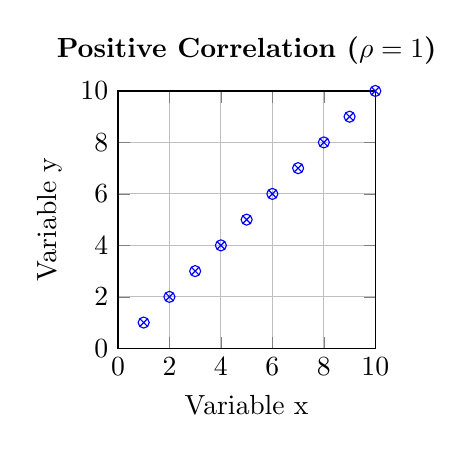
\begin{tikzpicture}
\begin{axis}[
    title={\textbf{Positive Correlation ($\rho = 1$)}},
    xlabel={Variable x},
    ylabel={Variable y},
    xmin=0, xmax=10,
    ymin=0, ymax=10,
    xtick={0,2,4,6,8,10},
    ytick={0,2,4,6,8,10},
    grid=major,
    legend pos=south east,
    width=0.4\textwidth,
    height=0.4\textwidth,
]
\addplot[
    only marks,
    mark=otimes,
    color=blue,
] coordinates {
(1,1)(2,2)(3,3)(4,4)(5,5)(6,6)(7,7)(8,8)(9,9)(10,10)
};
\end{axis}
\end{tikzpicture}
\hspace{1cm}
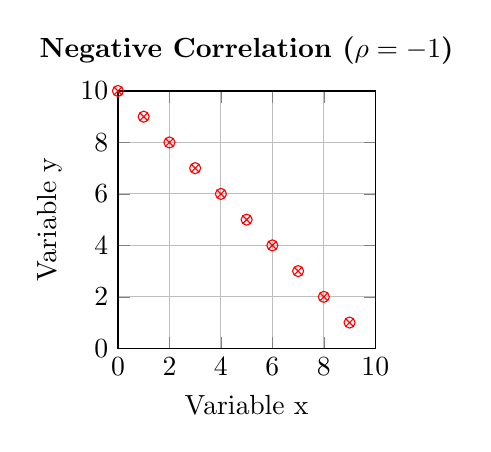
\begin{tikzpicture}
\begin{axis}[
    title={\textbf{Negative Correlation ($\rho = -1$)}},
    xlabel={Variable x},
    ylabel={Variable y},
    xmin=0, xmax=10,
    ymin=0, ymax=10,
    xtick={0,2,4,6,8,10},
    ytick={0,2,4,6,8,10},
    grid=major,
    legend pos=south east,
    width=0.4\textwidth,
    height=0.4\textwidth,
]
\addplot[
    only marks,
    mark=otimes,
    color=red,
] coordinates {
(9,1)(8,2)(7,3)(6,4)(5,5)(4,6)(3,7)(2,8)(1,9)(0,10)
};
\end{axis}
\end{tikzpicture}
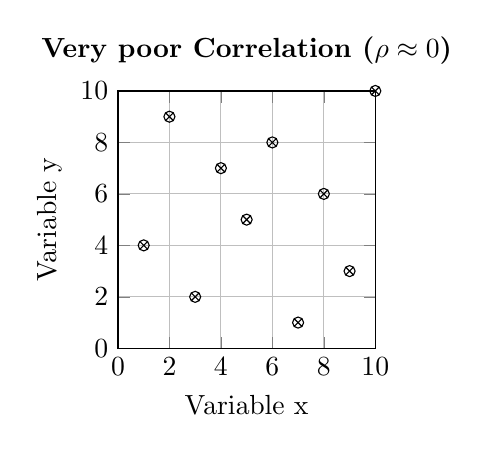
\begin{tikzpicture}
\begin{axis}[
    title={\textbf{Very poor Correlation ($\rho \approx 0$)}},
    xlabel={Variable x},
    ylabel={Variable y},
    xmin=0, xmax=10,
    ymin=0, ymax=10,
    xtick={0,2,4,6,8,10},
    ytick={0,2,4,6,8,10},
    grid=major,
    legend pos=south east,
    width=0.4\textwidth,
    height=0.4\textwidth,
]
\addplot[
    only marks,
    mark=otimes,
    color=black,
] coordinates {
(1,4)(2,9)(3,2)(4,7)(5,5)(6,8)(7,1)(8,6)(9,3)(10,10)
};
\end{axis}
\end{tikzpicture}

\caption{Scatter plots illustrating perfect positive, perfect negative correlations and very poor correlation}
\label{fig:correlations_illustrated}
\end{figure}

Spearman Rank Correlation works by calculating the difference in ranks of the two variables for each observation, then squaring these differences and summing them up, as given in \cref{eq:spearman}. 

\begin{equation} 
    \rho = 1 - \frac{6 \sum d_i^2}{n(n^2 - 1)}, 
    \label{eq:spearman}
 \end{equation}

where $d_i$ is the difference in ranks for each observation, and $n$ is the number of observations.

In the context of zero-cost proxies and validation accuracy, Spearman Rank Correlation can be used to determine whether there is a monotonic relationship between the two. A positive correlation would indicate that as the zero-cost proxy improves, so does the validation accuracy, while a negative correlation would imply an inverse relationship. A correlation near zero would suggest that the two variables have little or no association. 




\section{Exploration of Zero-Cost Proxies via Warmup Strategy}
\subsection{Theoretical and Practical Considerations}

\begin{comment}
    
The primary objective of \gls{NAS} is to discover high-performing architectures while minimising computational overhead. Training numerous architectures for a large number of epochs is computationally prohibitive. Training architectures for a limited number of epochs may be a more viable approach. In this context, we introduce the concept of a warmup strategy in this study, which aims to determine an optimal epoch threshold that can provide a reliable estimation of the relative performance of different architectures.
\end{comment}

In this section, we introduce the concept of a warmup strategy, which aims to determine an optimal epoch threshold that can provide a reliable estimation of the relative performance of different architectures. This contrast with the naive NAS approach of training numerous architectures, which can be computationally prohibitive. 

The underlying principle for this strategy is based on the assumption that training an architecture for $x$ epochs offers a more efficient evaluation than training the same architecture for $y$ epochs if $x < y$. By identifying an appropriate warmup threshold, researchers can effectively balance the trade-off between computational expense and the accuracy of architecture performance estimation.

To achieve this, each architecture is trained for a predetermined number of warmup epochs, and the zero-cost proxies are calculated at each epoch. Then, for every epoch, the Spearman Rank correlation coefficient between the zero-cost proxies and the final validation accuracy for all architectures is calculated. The epoch with the highest correlation is considered the optimal warmup point. 



\section{Combining Zero-Cost Proxies}

Upon analysing the outcomes derived from addressing research question 1 and research question 2, it became necessary to reconsider the experimental plan. The insights gained from the initial results prompted further exploration into utilising zero-cost proxies. Consequently, a decision was made to undertake additional ad hoc experiments to delve deeper into this area of investigation.



\subsection{Majority Vote Method}\label{subsec:vote}

The majority vote method, introduced by \cite{abdelfattah2021zero}, is an approach for ranking candidate architectures based on the pooled results of multiple zero-cost proxy metrics. This technique consolidates the rankings generated by different zero-cost proxy metrics, and the architectures are ranked according to the majority vote derived from these metrics. The algorithm of the voting method is outlined in \cref{alg:vote}. 

\begin{algorithm}[h!]
\caption{Voting Accuracy for Metric Combinations}\label{alg:vote}
\begin{algorithmic}[1]
\Function{vote}{$mets$, $gt$}
    \State $numpos \leftarrow 0$ \Comment{Initialize the number of positive elements}
    \For{each element $m$ in $mets$}
        \If{$m > 0$}
            \State Increment $numpos$ by 1
        \EndIf
    \EndFor
    \If{majority of elements in $mets$ are positive}
        \State $sign \leftarrow +1$
    \Else
        \State $sign \leftarrow -1$
    \EndIf
    \State \Return $sign * gt$ 
\EndFunction
\vspace{1em}
\Function{calc}{$acc$, $metrics$, $comb$}
    \State $num\_pts$ \Comment{Initialize the total number of data points }
    \State $tot \leftarrow 0$, $right \leftarrow 0$
    \For{each pair of distinct indices $i$ and $j$}
        \State $diff \leftarrow acc[i] - acc[j]$
        \If{$diff \neq 0$}
            \State $diffsyn$ \Comment{Initialize an empty list}
            \For{each metric $m$ in $comb$}
                \State $diffsyn \leftarrow metrics[m][i] - metrics[m][j]$
            \EndFor
            \State \textit{/* Check if $diffsyn$ and $diff$ have same sign */}
            \State $same\_sign \leftarrow$ \Call{vote}{$diffsyn$, $diff$}
            \If{$same\_sign > 0$}
                \State Increment $right$ 
            \EndIf
            \State Increment $tot$
        \EndIf
    \EndFor
    \State $votes \leftarrow \frac{right}{tot}$ \Comment{Calculate the voting accuracy}
    \State \Return $(comb, votes)$
\EndFunction
\end{algorithmic}
\end{algorithm}


Given that it is uncertain which combination of zero-cost proxies would yield the best results, the authors developed a function to generate all possible subsets of the 14 zero-cost proxy metrics. Subsequently, the majority vote for each subset was calculated and compared to the ground truth provided by the validation accuracy of every trained architecture in the benchmark. For example, \cref{tab:example_architectures} displays two architectures with given values for three zero-cost proxies (\gls{Synflow}, \gls{SNIP} and Grad Sign) and their validation accuracy. 

\begin{table}[h]
\centering
\caption{Example of two architectures with validation accuracy and zero-cost proxy metrics.}
\begin{tabular}{ll}
\textbf{Architecture} & \textbf{Metrics}          \\ \hline
\multicolumn{1}{l|}{1} & \multicolumn{1}{l}{Validation Accuracy: 0.85} \\
\multicolumn{1}{l|}{\cellcolor{verylightgray}} & \cellcolor{verylightgray}Synflow: 0.62 \\
\multicolumn{1}{l|}{} & \multicolumn{1}{l}{SNIP: 0.75} \\
\multicolumn{1}{l|}{\cellcolor{verylightgray}} & \cellcolor{verylightgray}Grad Sign: 0.28 \\ \hline
\multicolumn{1}{l|}{2} & \multicolumn{1}{l}{Validation Accuracy: 0.89} \\
\multicolumn{1}{l|}{\cellcolor{verylightgray}} & \cellcolor{verylightgray}Synflow: 0.48 \\
\multicolumn{1}{l|}{} & \multicolumn{1}{l}{SNIP: 0.82} \\
\multicolumn{1}{l|}{\cellcolor{verylightgray}} & \cellcolor{verylightgray}Grad Sign: 0.36
\end{tabular}
\label{tab:example_architectures}
\end{table}

By examining the validation accuracy, one can deduce that Architecture 2 is superior to Architecture 1. Upon analysing the computed zero-cost proxy metrics, the following observations can be made:

\begin{itemize}
\item \textbf{Synflow}: Architecture 1 $(0.62) >$ Architecture 2 $(0.48)$
\item \textbf{SNIP}: Architecture 1 $(0.75) <$ Architecture 2 $(0.82)$
\item \textbf{GradSign}: Architecture 1 $(0.28) <$ Architecture 2 $(0.36)$
\end{itemize}

In this case, one positive difference (\gls{Synflow}) and two negative differences (\gls{SNIP} and Grad Sign). Consequently, the majority vote favours Architecture 2, consistent with the validation accuracy.

\subsection{Weighted Arithmetic Mean}
The weighted arithmetic mean, as described in \autocite{wam}, is a widely used technique in statistics and data analysis. This study applied the weighted arithmetic mean method to the zero-cost proxies using Spearman's rank correlation as weights for ranking various architectures.

\begin{algorithm}
\caption{Weighted Arithmetic Mean for datapoint $d$}\label{alg:weighted_mean}
\begin{algorithmic}[1]
\Require Zero-cost proxies $P_d = \{p_1, p_2, \dots, p_n\}$
\Require Validation accuracy $A_d$
\State Normalise zero-cost proxies: $P_{d_{norm}} = \{p_{1_{norm}}, p_{2_{norm}}, \dots, p_{n_{norm}}\}$
\For{$i = 1$ to $n$}
    \State Calculate Spearman's rank correlation $r_i$ between $p_{i_{norm}}$ and $A_d$
    \State Assign weight $w_i = r_i$
\EndFor
\State Initialize: $\text{Score}_d \leftarrow 0$, $total\_weight \leftarrow 0$
\For{$i = 1$ to $n$}
    \State $\text{Score}_d \leftarrow \text{Score}_d + (p_{i_{norm}} * w_i)$
    \State $total\_weight \leftarrow total\_weight + w_i$
\EndFor
\State $\text{Score}_d \leftarrow \frac{\text{Score}_d}{total\_weight}$
\State Calculate correlation between $\text{Score}_d$ and $A_d$ using Spearman's rank correlation
\end{algorithmic}
\end{algorithm}


As illustrated in \cref{alg:weighted_mean}, each zero-cost proxy value is first normalised with min-max normalisation, ensuring they are on a comparable scale for accurate comparison and combination. Next, weights were assigned to each zero-cost proxy based on their performance. Finally, Spearman's rank correlation evaluated the correlation between each proxy and the validation accuracy. Higher correlation values indicated better performance and proxies with stronger correlations received larger weights.

For the weighted arithmetic mean calculation, the normalised value of each zero-cost proxy was multiplied by its respective weight for every data point, and the products were summed. The combined score was then calculated by dividing the sum of these products by the total sum of the weights using the formula: 
\begin{equation*} 
    \text{Score} = \frac{\sum x_i * w_i }{\sum w_i}, 
\end{equation*} 
where $w_i$ is the weight assigned to the $\text{i-th}$ zero-cost proxy, $x_i$ represents the normalised value of the $\text{i-th}$ zero-cost proxy. The sums are calculated using all zero-cost proxies.

After obtaining the combined scores, the architectures were ranked based on these scores, with higher scores indicating better-performing architectures. Finally, the effectiveness of the weighted arithmetic mean approach was evaluated by calculating the correlation between the weighted arithmetic mean score and the validation accuracy using Spearman's rank correlation coefficient.
\chapter{Results}\label{results}
\begin{comment}
In this chapter, we present the results of our investigation into the use of zero-cost proxies in neural architecture search (NAS) for graph convolutional networks (GCN). We address three research questions about using proxies in NAS for GCN, as outlined in the introduction chapter (\ref{section:goalsandrq}). Specifically, we analyze the effectiveness of different zero-cost proxies in ranking GCN architectures, examine the impact of incorporating proxies in the NAS algorithm and investigate the effectiveness of using an ensemble of proxies in NAS.
\end{comment}

\begin{comment}
Chapter 5 of the thesis presents the results of an investigation into the use of zero-cost proxies in neural architecture search for graph convolutional networks. The chapter includes a section on correlation and a vote section that analyze the effectiveness of different zero-cost proxies in ranking GCN architectures. Additionally, a section on supervised learning using Recursive Feature Elimination with Cross-Validation and Pointwise Ranking with Regression and Cross-Validation is included. Finally, the chapter addresses three research questions about the use of proxies in NAS for GCN and examines the impact of incorporating proxies in the NAS algorithm and investigates the effectiveness of using an ensemble of proxies in NAS.
\end{comment}

This chapter outlines the study's findings, responding to the defined research questions. Next, the 'Correlation Analysis' section evaluates the capability of zero-cost proxies in ranking GCN architectures concerning their validation accuracy. Subsequently, the analysis of correlation during the warm-up phase of GCN training is identified. Lastly, the 'Vote' and 'Weighted Arithmetic Mean' section examines techniques for combining zero-cost proxies to improve efficiency and accuracy in NAS algorithms.


\section{Correlation Analysis}\label{res:correlation}

Establishing a benchmark provided the foundation for investigating the correlation between various zero-cost proxies and the ground truth represented by the validation accuracy. The Spearman Rank Correlation was employed to measure the correlation, as discussed in \cref{sec:corr}. 

\Cref{tab:corr} displays the obtained results, utilising the 693 architectures derived from the created benchmark. 
\clearpage

\begin{table}[h]
\caption{Correlation coefficients between proxy scores and model performance before training}
\centering
\begin{tabular}{lr}
\textbf{Name} & \textbf{$\rho$} \\ \hline
\multicolumn{1}{l|}{\cellcolor{verylightgray}epe\_nas} & \cellcolor{verylightgray}$0.0090$ \\
\multicolumn{1}{l|}{fisher} & $0.2405$ \\
\multicolumn{1}{l|}{\cellcolor{verylightgray}flops} & \cellcolor{verylightgray}$0.7241$ \\
\multicolumn{1}{l|}{grad\_norm} & $0.2653$ \\
\multicolumn{1}{l|}{\cellcolor{verylightgray}grad\_sign} & \cellcolor{verylightgray}$0.4979$ \\
\multicolumn{1}{l|}{grasp} & $-0.4244$ \\
\multicolumn{1}{l|}{\cellcolor{verylightgray}jacov} & \cellcolor{verylightgray}$-0.0465$ \\
\multicolumn{1}{l|}{l2\_norm} & $0.7325$ \\
\multicolumn{1}{l|}{\cellcolor{verylightgray}nwot} & \cellcolor{verylightgray}$0.1214$ \\
\multicolumn{1}{l|}{params} & $0.6164$ \\
\multicolumn{1}{l|}{\cellcolor{verylightgray}plain} & \cellcolor{verylightgray}$0.2490$ \\
\multicolumn{1}{l|}{snip} & $0.2468$ \\
\multicolumn{1}{l|}{\cellcolor{verylightgray}synflow} & \cellcolor{verylightgray}0.7599 \\
\multicolumn{1}{l|}{zen} & \textbf{0.7827} \\
\end{tabular}
\label{tab:corr}
\end{table}



The results in \cref{tab:corr} reveal that specific proxies correlate strongly with the validation accuracy, while others demonstrate weaker correlations. \Cref{tab:corr} indices that Zen has the highest correlation with model performance, with a coefficient of $0.7827$. \gls{Synflow} is also performing well, with a coefficient of $0.7599$. This suggests that Zen and \gls{Synflow} are the most effective zero-cost proxies among the ones considered in this study. 

Conversely, the epe\_nas and jacov proxies exhibit a weak correlation with the model performance, with coefficients of $0.0090$ and $-0.0465$, respectively. 

It is also worth noting that the l2\_norm, \gls{FLOPs}, and params proxies show relatively strong correlations with coefficients of $0.7325$, $0.7241$, and $0.6164$, respectively. Although these proxies might be less effective than Zen and \gls{Synflow}, they still demonstrate considerable potential for predicting model performance.

The findings of this correlation analysis provide valuable insights into the predictive capacity of each proxy in relation to the ground truth. This understanding can inform the development of more efficient and effective \gls{NAS} approaches, thereby reducing computational demands and enabling more rapid progress in the field.

\subsection{Vote}




After sorting, the results will only display the top-5 combinations as too many values will be shown. However, from the results shown in \cref{tab:vote}, all combinations of metrics exhibit almost the same custom correlation measure (majority vote score) of $ > 0.788$. This suggests that these combinations of metrics perform similarly in terms of the agreement between the majority of metrics and accuracy differences.

\begin{table}[h!]
\caption{Vote scores}
\centering
\begin{tabular}{ll}
\textbf{Name} & \textbf{Value} \\ \hline
\multicolumn{1}{l|}{synflow, zen, fisher} & \textbf{0.7899} \\
\multicolumn{1}{l|}{\cellcolor{verylightgray}synflow, zen, nwot} & \cellcolor{verylightgray}$0.7888$ \\
\multicolumn{1}{l|}{synflow, zen, flops} & $0.7885$ \\
\multicolumn{1}{l|}{\cellcolor{verylightgray}synflow, zen, plain} & \cellcolor{verylightgray}$0.7883$ \\
\multicolumn{1}{l|}{synflow, zen, grad\_norm} & $0.7883$ \\
\end{tabular}
\label{tab:vote}
\end{table}

It is important to note that these results are based on the custom correlation measure (see \cref{subsec:vote}), which differs from standard correlation measures such as Spearman's rank correlation. The custom correlation measure captures the extent to which the majority of metric differences agree with the differences in dataset accuracies. A higher correlation value indicates a stronger agreement, while a lower correlation value suggests a weaker agreement.

\subsection{Warmup}

\Cref{fig:warmup,fig:warmup_seperate} presents the variation in correlation during the initial ten epochs, with epoch -1 representing the starting correlations (same as \cref{tab:corr}). As shown in the figures, \gls{Synflow} and Zen exhibit the highest performance, maintaining a stable correlation at $\approx 0.8$ throughout the observed epochs. A minor increment in correlation can be observed, although its impact is relatively insignificant. Furthermore, Params, L2-norm, and \gls{FLOPs} exhibit consistently strong performance with a correlation coefficient ($\rho$) exceeding $0.6$ across all epochs under consideration.

\begin{figure}[!ht]
  \centering
  \includesvg[width=0.8\columnwidth]{figures/correlations.svg}
  \caption{Correlations for all zero-cost proxies over multiple epochs}
  \label{fig:warmup}
\end{figure}

\clearpage

\begin{figure}[htbp]
  \centering
    \begin{adjustbox}{width=1.2\columnwidth,center}
  \begin{tabular}{ccc}
    \includesvg[width=0.5\textwidth]{figures/correlations/epe_nas_correlations.svg} &
    \includesvg[width=0.5\textwidth]{figures/correlations/fisher_correlations.svg} &
    \includesvg[width=0.5\textwidth]{figures/correlations/flops_correlations.svg} \\
    \includesvg[width=0.5\textwidth]{figures/correlations/grad_norm_correlations.svg} &
    \includesvg[width=0.5\textwidth]{figures/correlations/grad_sign_correlations.svg} &
    \includesvg[width=0.5\textwidth]{figures/correlations/grasp_correlations.svg} \\
    \includesvg[width=0.5\textwidth]{figures/correlations/jacov_correlations.svg} &
    \includesvg[width=0.5\textwidth]{figures/correlations/l2_norm_correlations.svg} &
    \includesvg[width=0.5\textwidth]{figures/correlations/nwot_correlations.svg} \\
    \includesvg[width=0.5\textwidth]{figures/correlations/params_correlations.svg} &
    \includesvg[width=0.5\textwidth]{figures/correlations/plain_correlations.svg} &
    \includesvg[width=0.5\textwidth]{figures/correlations/snip_correlations.svg} \\
    \includesvg[width=0.5\textwidth]{figures/correlations/synflow_correlations.svg} &
    \includesvg[width=0.5\textwidth]{figures/correlations/zen_correlations.svg} 
  \end{tabular}
  \end{adjustbox}
  \caption{Each zero-cost proxy with the correlation over multiple epochs}
  \label{fig:warmup_seperate}
\end{figure}

\section{Weighted Arithmetic Mean}

\Cref{fig:weighted} displays a scatter plot illustrating the relationship between validation accuracy and the weighted arithmetic mean. Every data point displayed within the graph corresponds to a unique architecture evaluated during the experiment. A dotted red line represents the best-fit linear regression line through the data points. Additionally, the graph includes Spearman's rank correlation coefficient in the title, which measures the monotonic relationship between the validation accuracy and the weighted arithmetic mean. 

\begin{figure}[h!]
  \centering
  \includesvg[width=0.9\columnwidth]{figures/weighted_average.svg}
  \caption{Weighted Arithmetic Mean}
  \label{fig:weighted}
\end{figure}



%
\section{Supervised Learning}
\subsection{Recursive Feature Elimination with Cross-Validation}
This section presents the feature selection results using Recursive Feature Elimination with Cross-Validation (RFECV) and its impact on the model's performance. Our initial dataset consists of 14 zero-cost proxy features, and our goal is to identify the optimal subset of features that would lead to the highest R2 score in our regression model.

We employed the RFECV algorithm for feature selection, which iteratively eliminates the least essential features from the dataset based on their importance, as determined by the model's coefficients or feature importances. The model performance is evaluated using cross-validation at each iteration, and the optimal number of features is chosen based on the highest R2 score.

Upon applying the RFECV algorithm, only one feature was selected as optimal, implying that this single feature provides the highest R2 score during cross-validation. However, the resulting R2 score on the test set is 0.14, indicating that the selected feature explains only a tiny portion of the variance in the target variable.

\subsection{Pointwise Ranking with Regression and Cross-Validation}

\kommentar{Hvor er det mentioned??}{}

As mentioned in \cref{}, one approach used supervised learning with pointwise ranking and cross-validation to assess the performance of combining zero-cost proxies. Our analysis involved training a linear regression model to predict the performance of various \gls{GCN} architectures based on the combined zero-cost proxy features. We then ranked the architectures based on their predicted performance scores and evaluated the ranking quality using measures such as Mean Squared Error (MSE) and Normalized Discounted Cumulative Gain (NDCG). The results are presented for the approach without cross-validation and the refined approach with cross-validation.

\begin{table}[h]
\centering
\begin{tabular}{ll}
\textbf{Evaluation Method}             & \textbf{Mean Squared Error} \\ \hline
\multicolumn{1}{l|}{Without Cross-Validation} & 0.00108281          \\
\multicolumn{1}{l|}{\cellcolor{verylightgray}With Cross-Validation} & \cellcolor{verylightgray}0.00145585 \\ \hline
\end{tabular}
\begin{tabular}{ll}
\textbf{Evaluation Method}             & \textbf{NDCG} \\ \hline
\multicolumn{1}{l|}{Without Cross-Validation} & 0.9999999999999997          \\
\multicolumn{1}{l|}{\cellcolor{verylightgray}With Cross-Validation} & \cellcolor{verylightgray}0.9999999999999997 \\ \hline
\end{tabular}
\caption{Comparison of pointwise ranking results with and without cross-validation}
\label{tab:ranking_results}
\end{table}


\Cref{tab:ranking_results} summarizes the results of our experiments. The Mean Squared Error (MSE) and Normalized Discounted Cumulative Gain (NDCG) scores are reported for both the original approach without cross-validation and the approach with cross-validation.

Without cross-validation, the model achieved an MSE of 0.00108281 and an NDCG score of 0.9999999999999997. When using cross-validation, the model achieved an MSE of 0.00145585 and an NDCG score of 0.9999999999999997 (averaged over cross-validation folds).




\chapter{Discussion}\label{discussion}
\begin{comment}
This chapter aims to analyse and interpret the findings of our study in the context of the overall goal and research questions. Our research aimed to improve and optimise the efficiency of neural architecture search (NAS) with graph convolutional networks (GCN) for human action recognition (HAR). The authors will first interpret the results of each research question and discuss their implications in the context of the overall goal. We will then consider the significance of our findings and their potential impact on the field of NAS with GCN for HAR. Furthermore, we will acknowledge the limitations of our study. 
\end{comment}
Chapter 6 of the thesis discusses the study's findings on improving and optimising the efficiency of NAS with GCN for HAR. The chapter aims to analyse and interpret the results of each research question and their implications in the context of the overall goal. The authors also discuss the significance and potential impact of the findings on the field of NAS with GCN for HAR and acknowledge the study's limitations. In addition, a discussion on the overall environmental implication is included. 

\begin{comment}
    In this chapter, the method and experimental result are analysed and discussed regarding
their merits and limitations in light of research from the literature. The chapter is
concluded with a discussion of how the research questions are answered.
\end{comment}
\section{Interpretation and Significance of Results}

\subsection{RQ1 How well can different zero-cost proxies rank GCN architectures compare to their validation accuracy?}

\Cref{res:correlation} highlights the results for the given research question in which the correlation between the different zero-cost proxies and the validation accuracy is presented. Positive correlation values indicate that as the proxy metric increases, the validation accuracy also increases, whereas negative values indicate the opposite. The magnitude and sign of the Spearman rank correlation coefficient, also known as Spearman's rho (\(\rho\)), can be used to interpret the strength and direction of the association between two ranked variables \autocite{pallant2016spss}.

According to \cite{spear}, Spearman's correlation can generally be described using the following guidelines:

\begin{table}[h]
\caption{Guidelines for interpreting Spearman's correlation}
\centering
\begin{tabular}{lc}
\textbf{Correlation coefficient} & \textbf{Strength of correlation} \\ \hline
\multicolumn{1}{l|}{.00-.19} & Very weak \\
\multicolumn{1}{l|}{\cellcolor{verylightgray}.20-.39} & \cellcolor{verylightgray}Weak \\
\multicolumn{1}{l|}{.40-.59} & Moderate \\
\multicolumn{1}{l|}{\cellcolor{verylightgray}.60-.79} & \cellcolor{verylightgray}Strong \\
\multicolumn{1}{l|}{.80-1.0} & Very strong \\
\end{tabular}
\label{tab:correlation}
\end{table}

The results showed that zen and \gls{Synflow} performed the best with a spearman $\rho$ of $0.7827$ and $0.7599$, respectively. This is a very strong correlation, as indicated by \cite{spear}, demonstrating that the zero-cost proxies can confidently predict model performance without incurring significant computational overhead. The strength of these correlations suggests that both zen and \gls{Synflow} effectively capture fundamental architectural and optimisation properties critical for achieving high validation accuracy in neural networks. Furthermore, given the variations in the validation accuracy in the benchmark $[0.92 - 0.95]$, and the provided correlations, both \gls{Synflow} and Zen are sensitive to subtle differences in performance among the models, effectively ranking them based on their validation accuracy. 

For comparison, \cite{abdelfattah2021zero} reported the following results of zero-cost proxies on NAS-Bench 201. Note here that this is a benchmark for a different task. 

\begin{table}[h]
\caption{Comparison of various methods on different datasets}
\centering
\begin{adjustbox}{center}
\begin{tabular}{l|cccccc}
\textbf{Dataset} & \textbf{grad\_norm} & \textbf{snip} & \textbf{grasp} & \textbf{fisher} & \textbf{synflow} & \textbf{jacob\_cov} \\ \hline
\multicolumn{1}{l|}{CIFAR-10} & 0.58 & 0.58 & 0.48 & 0.36 & 0.74 & 0.73 \\
\multicolumn{1}{l|}{\cellcolor{verylightgray}CIFAR-100} & \cellcolor{verylightgray}0.64 & \cellcolor{verylightgray}0.63 & \cellcolor{verylightgray}0.54 & \cellcolor{verylightgray}0.39 & \cellcolor{verylightgray}0.76 & \cellcolor{verylightgray}0.71 \\
\multicolumn{1}{l|}{ImageNet16-120} & 0.58 & 0.58 & 0.56 & 0.33 & 0.75 & 0.71 \\
\end{tabular}
\end{adjustbox}
\label{tab:comparison}
\end{table}

The results in \cref{tab:comparison} from \cite{abdelfattah2021zero} show that the performance of the zero-cost proxies varies across different datasets. It is important to note that \gls{NAS}-Bench 201 is a different benchmark and has other properties than the dataset used in this study. Nonetheless, a comparison can provide valuable insights into the generalisability and robustness of these methods across various tasks.

From \cref{tab:comparison}, it is evident that \gls{Synflow} performs consistently well across all three datasets, with correlation coefficients of 0.74, 0.76, and 0.75 for CIFAR-10, CIFAR-100, and ImageNet16-120, respectively. The results support the thesis' finding that \gls{Synflow} is a reliable and robust predictor of model performance. Similarly, grad\_norm and \gls{SNIP} exhibit relatively high correlations across the datasets, although not as strong as \gls{Synflow}. This suggests that these methods may also provide valuable information when predicting model performance but with varying effectiveness.

The practical implications of this thesis's findings suggest that \gls{Synflow} and zen could be valuable components of a \gls{NAS} algorithm in the context of \gls{GCN} for \gls{HAR} tasks, given their strong correlations with model performance. However, it is essential to note that the current study utilised a specific framework designed for \gls{GCN} \gls{HAR} tasks with the NTU RGB+D dataset. This means that the demonstrated efficiency of using zero-cost proxies, such as \gls{Synflow} and zen, is effective for this case.

However, the generalisability of these results to other tasks, datasets, or frameworks remains to be established. Further research is needed to assess the effectiveness and applicability of \gls{Synflow}, zen, and other zero-cost proxies across a broader range of neural network architectures and tasks. By doing so, the academic community can better understand the potential benefits and limitations of incorporating zero-cost proxies into \gls{NAS} algorithms for various problem domains.  

The significance of these findings lies in their potential to improve the efficiency and effectiveness of \gls{NAS} methods by identifying zero-cost proxies with solid predictive capacities. Furthermore, by understanding which proxies are more reliable in ranking \gls{GCN} architectures to their validation accuracy, researchers can prioritise their use in \gls{NAS} algorithms and reduce the overall computational demands of the architecture search process.

This is particularly important given neural networks' growing scale and complexity, often requiring substantial computational resources to explore and evaluate. Focusing on zero-cost proxies with strong correlations can significantly reduce the search space and the time required to identify optimal architectures.

Furthermore, these findings stimulate additional research into developing and refining zero-cost proxies that exhibit stronger correlations with validation accuracy. This could lead to the discovery of new proxies that further improve the efficiency and accuracy of \gls{NAS} methods, thus accelerating progress in the field.

Finally, the reduced computational demands also result in lessening the environmental impact. By decreasing the training time and computational resources required for \gls{NAS}, one can significantly lower the process's energy consumption and associated carbon footprint. This aligns with the growing global concern for sustainable practices in artificial intelligence research and development.


\subsection{RQ2 How early can we identify the correlation between zero-cost proxies and validation accuracy during the warmup phase of GCN training in order to potentially halt the training process sooner?}

The results presented in \cref{results} provide valuable insights into how the relationship between zero-cost proxies and validation accuracy evolves during the warmup phase of \gls{GCN} training. By analysing the Spearman Rank correlation coefficients between the 14 proxies and the model performance for each epoch (see \cref{fig:warmup}), one can determine the optimal warmup point for each architecture.

The correlation coefficients reveal that some zero-cost proxies, such as \gls{Synflow}, flops, params, and l2\_norm, consistently show strong positive correlations with the validation accuracy throughout the warmup phase. On the other hand, some proxies, like \gls{GRASP}, grad\_sign, and jacov, display weak or negative correlations. This suggests that specific zero-cost proxies are more reliable indicators of an architecture's potential performance.

Moreover, the optimal warmup points vary across the different zero-cost proxies, as evident from the highest correlation coefficients achieved at different epochs. For example, \gls{Synflow} achieves its highest correlation at epoch 8, while l2\_norm peaks at initialisation. This indicates that there is no optimal warmup point for all proxies, and the choice of a warmup point depends on the specific proxy used for performance estimation.

The significance of the results is that there is no improvement in using warmup regarding the correlation and that the zero-cost proxies are most effective when the network is initialised. From an academic perspective, it is crucial to note this study's implications on \gls{NAS} algorithms. The findings suggest that the necessity of training architectures within a \gls{NAS} algorithm may be an oversimplified assumption. Given that zero-cost proxies were found to be most effective at the initialisation stage, one can assume that the requirement of training architectures may be less vital to the successful implementation of a \gls{NAS} algorithm than previously believed.

\subsection{RQ3 How can we effectively combine zero-cost proxies using various techniques to enhance the efficiency and accuracy of architecture search in Neural Architecture Search (NAS) algorithms?}

\cite{colin2022adeeperlook} argued that zero-cost proxies have untapped potential and referred to preliminary research, which showed zero-cost proxies shine when combined rather than individually. How to combine them is another question that one should raise, as there are many different opportunities to discover. This study investigated the effectiveness of combining zero-cost proxies to improve the efficiency and accuracy of architecture search in \gls{NAS} algorithms, as posed in Research Question 3. 

Considering the high Spearman's rank correlation for zen and \gls{Synflow}, combining methods has little room for improvement, as the correlation is already strong. It is important to note that using the majority vote and weighted arithmetic mean helps maximise the different metrics' variety to create a better correlation. With this in mind, and looking at \cref{fig:weighted}, there is a positive link between validation accuracy and the weighted arithmetic mean, shown by the upward slope of the best-fit line. This means architectures with higher validation accuracy usually have higher weighted arithmetic means. Spearman's rank correlation coefficient of $0.766$ supports this idea, showing a strong positive relationship between the two factors. Combining methods like the weighted arithmetic mean makes a more stable metric that benefits from the variation among different metrics while still focusing on the better-performing proxies. These results suggest that exploring and improving these methods could be valuable for future research in architectural evaluation, even though there is no concrete improvement in using the zero-cost proxies individually. 

The presented methods in this study are relatively simple yet efficient methods discovered. However, various other methods can be explored for combining zero-cost proxies. One approach is supervised learning,  which involves training a model on labelled input-output pairs to learn the underlying relationship between input features and target outputs. An approach in the context of \gls{NAS} is developing a machine learning model specifically designed to learn how to rank architectures, utilising zero-cost proxies as input features. This method aims to leverage the information the zero-cost proxies provide to establish a relative ranking of architectures, guiding the search process towards the most promising candidates effectively and efficiently. 

RankNet is a pairwise ranking model based on a neural network architecture proposed by \cite{burges2005learning} in the paper Learning to rank using gradient descent. The model is designed to learn how to rank entities by minimising a pairwise loss function, typically using cross-entropy loss or a variant thereof. The core idea behind RankNet is to represent entities using input features and predict their relative ranking based on pairwise comparisons. During training, the model receives pairs of entities represented by their respective feature vectors and learns the underlying relationship between these features and the desired ranking. The training data includes binary labels indicating which entity in a pair is superior based on their ranking.

Applying RankNet to \gls{NAS} algorithms offers several advantages. First, by leveraging the pairwise ranking approach, RankNet allows for a more nuanced understanding of the relative performance of different architectures based on their zero-cost proxies. This is particularly beneficial in the context of \gls{NAS}, where the search space is vast and evaluating each architecture based on its actual performance is computationally expensive.

Furthermore, by training a neural network to learn the relationships between zero-cost proxies and architecture performance, RankNet has the potential to uncover hidden patterns and interactions among these proxies that may not be immediately evident. This can lead to a more accurate and efficient ranking of candidate architectures, reducing the search time and computational resources required for \gls{NAS}.



%\section{Significance of Results}

Discuss the importance of your findings and their potential impact on the field of neural architecture search with graph convolutional networks for human action recognition. Consider the practical implications of using zero-cost proxies for ranking \gls{GCN} architectures and in a warm-up approach.

\begin{comment}
\subsection{RQ1:}

Har lagt til dette i første kap om RQ 1. 
\end{comment}
\begin{comment}
\subsection{RQ2:}
The findings from this study carry significant implications for the field of \gls{NAS}, particularly in terms of performance estimation and computational efficiency working with \gls{GCN}. By identifying the optimal warm-up points for different zero-cost proxies, we can potentially halt the training process much earlier than traditionally done, without sacrificing the accuracy and reliability of performance estimation.

This early stopping of training can lead to substantial reductions in computational workload and search costs, making the \gls{NAS} process more efficient and accessible to a wider range of researchers and practitioners. Additionally, the improved performance prediction facilitated by the warm-up phase enables more effective exploration of the search space in \gls{NAS}, leading to the discovery of better architectures. 

Notably, the reduced computational demands also result lessening the environmental impact. By decreasing the training time and computational resources required for \gls{NAS}, we can significantly lower the energy consumption and the associated carbon footprint of the process. This aligns with the growing global concern for sustainable practices in artificial intelligence research and development.

In conclusion, the results of this study provide a solid foundation for further research into the application of warm-up with zero-cost proxies in \gls{NAS}. Future studies could investigate the generalizability of these findings across different datasets and tasks or explore ways to combine multiple zero-cost proxies for even more accurate and reliable performance estimation.

\end{comment}
\begin{comment}
\subsection{RQ3:}

The results of this study have significant implications for the field of Neural Architecture Search (\gls{NAS}) and its applications. By effectively combining zero-cost proxies, we can improve the efficiency and accuracy of architecture search, thus reducing the computational demands and enabling more rapid progress in the field. By guiding the \gls{NAS} algorithms towards more promising regions of the search space, researchers can develop better-performing neural network architectures, which in turn can be applied to various real-world problems, such as image recognition, natural language processing, and more.

Furthermore, the study provides insights into the predictive capacity of each individual proxy in relation to the ground truth (validation accuracy). This understanding can inform the development of more efficient and effective \gls{NAS} approaches by focusing on the most predictive zero-cost proxies.

\section{Alternative Methods and Future Directions}

While the majority vote method and the weighted arithmetic mean method have proven to be effective in this study, other techniques could be explored in future research to further enhance the efficiency and accuracy of architecture search in \gls{NAS} algorithms.

One such approach is the use of supervised learning models, such as neural networks or decision trees, to combine the zero-cost proxies. These models could be trained on a set of candidate architectures, with their zero-cost proxy metrics as features and their validation accuracy as the target variable. Once trained, these models could be employed to predict the performance of untrained architectures based on their zero-cost proxy metrics, thus providing a more efficient means of ranking candidate architectures.

Furthermore, an unsupervised learning approach, such as clustering, could be employed to group candidate architectures based on their zero-cost proxy metrics. By identifying clusters of architectures with similar performance characteristics, \gls{NAS} algorithms could be guided towards more promising regions of the search space, potentially improving search efficiency.

Another avenue for future research is the development of new zero-cost proxy metrics that better capture the performance characteristics of neural networks. By identifying metrics with stronger correlations to validation accuracy, the efficacy of combined zero-cost proxy metrics can be further improved.
\end{comment}
\section{Limitations}
\subsection{Dataset size}

One of the main limitations of this study is the relatively small dataset size. Comparable studies like \autocite{abdelfattah2021zero, colin2022adeeperlook} used state-of-the-art benchmarks consisting of thousands of fully trained architectures. The developed dataset in this thesis consists of 693 trained architectures, each with their respective validation accuracy. For each architecture, the score of 14 different zero-cost proxies is calculated and then used for various analyses, such as determining the correlation between the proxies and the validation accuracy.

Although this dataset provides insights into the relationship between zero-cost proxies and the performance of \gls{GCN} models within \gls{HAR} tasks, the small number of trained architectures may limit the generalisability of the findings. A larger dataset with more architectures could reveal more subtle relationships between the proxies and the validation accuracy, leading to more accurate conclusions.

The relatively small dataset size may also affect the statistical significance of our results. With a larger dataset, one could observe stronger correlations between the zero-cost proxies and the validation accuracy, strengthening the validity of our conclusions. Additionally, a larger dataset would allow for a more robust exploration of potential relationships between different architectures and proxy scores.

Future work should expand the dataset to address these limitations by incorporating more trained architectures with varying characteristics. This would increase the generalisability of the findings and enable a more comprehensive understanding of the relationships between zero-cost proxies and the performance of \gls{GCN} models within \gls{HAR} tasks.


\subsection{Limitations of Relying Solely on the GCN-NAS Framework for NAS Acceleration}

Using the \gls{GCN}-\gls{NAS} framework for developing a \gls{NAS} acceleration technique for \glspl{GCN} offers a valuable starting point. However, focusing exclusively on this framework introduces limitations that may affect the \gls{NAS} acceleration approach's generalisability, robustness, and thoroughness. This section will present a discussion of these limitations and their potential impact on the applicability of the acceleration technique to other \gls{GCN}-\gls{NAS} frameworks.

\subsubsection{Limited Generalisability}
By concentrating on the \gls{GCN}-\gls{NAS} framework, the developed \gls{NAS} acceleration technique may become tailored to the specific characteristics of this framework, thereby restricting its generalisability to other \gls{GCN}-\gls{NAS} frameworks. This limitation could compromise the effectiveness of the acceleration method when applied to alternative \gls{GCN}-\gls{NAS} frameworks with different search spaces, function modules, or optimisation techniques.

\subsubsection{Lack of Comparative Analysis}
The unavailability of multiple \gls{GCN}-\gls{NAS} frameworks for evaluation prevents a comprehensive comparative analysis, making it challenging to identify the relative strengths and weaknesses of the proposed \gls{NAS} acceleration technique. However, with the ability to compare performance across frameworks, pinpointing areas of improvement or potential pitfalls in the acceleration method becomes more effortless. 

It should be noted that an attempt to implement the Zero-Cost Framework (\cref{sec:zc-framework}) into a new \gls{GCN}-\gls{NAS} framework developed by the InMotion team at \gls{NTNU} and St. Olavs Hospital was conducted. However, as this is outside this thesis's scope and due to time limitations, the results are not included. However, the initial experiments show that $ \rho >0.8$ score for multiple proxies. The \gls{GCN}-\gls{NAS} framework is still under development and can be explored further when completed. The initial results can be found in Appendix X. 


    
\subsubsection{Difficulty in Validating Robustness}

Evaluating the zero-cost proxies on a single \gls{GCN}-\gls{NAS} framework restricts the ability to assess the technique's robustness. The proxies should be tested across multiple frameworks to determine their adaptability to various search spaces, hyperparameter configurations, and problem domains. This lack of validation can lead to overestimating the technique's performance, potentially concealing its weaknesses.

Future research could consider utilising multiple \gls{GCN}-\gls{NAS} frameworks to address these limitations, exploring diverse search strategies and validating the acceleration technique across different problem domains. 

\section{Environmental Implications}
\subsection{Energy consumption / Creating benchmark}

As elaborated in \cref{subsec:experimentalsetup}, 693 neural network architectures were trained and evaluated to obtain their validation accuracy for later use in experiments. The training process required a significant investment of computational resources, and multiple \glspl{GPU} were used to complete the training. A Python script was utilised to capture the total training time in seconds to measure the training time for each architecture accurately.

\begin{equation*} 32833726.233713627 \div 3600 = 9120.4795093649 \end{equation*}

\begin{equation*}
    9120.4795093649 \div 24 = 380
\end{equation*}

So in total, 380 \gls{GPU} days were used to obtain the benchmark for the experiments. 

For contextual comparison, NASBench-101 is a benchmark for \gls{NAS} introduced by \autocite{ying2019bench}. The benchmark contains many \gls{CNN} architectures trained and evaluated on the CIFAR-10 dataset using over 100 TPU \footnote{Tensor Processing Unit introduced by Google purposely designed for machine learning workloads} years of computation time. 

\subsection{Reduced Search Time and Future Benefits}

\begin{comment}
\begin{itemize}
    \item Discuss how this approach might reduce the time spent on neural architecture search
    \item Address the broader implications of such reductions, such as enabling more efficient research, reducing the overall environmental impact of the field, and making neural architecture search more accessible to researchers with limited resources.
\end{itemize}
\end{comment}

Creating a benchmark involves substantial time and energy investments, as demonstrated in this study and other benchmarks \autocite{dong2020bench, ying2019bench, tu2021bench}. In addition, training and evaluating diverse neural network architectures requires significant computational resources, leading to increased energy consumption and longer training durations. Therefore, although the research required a considerable investment in \gls{GPU} days, the long-term benefits of this investment should be considered. 

The most naive approach for any general \gls{NAS} algorithm is to generate a set of candidate architectures, train them until convergence, and find the best-performing architecture. However, this approach is computationally infeasible when the search space is ample. In addition, this specific approach exhibits a substantial carbon footprint because of its extensive usage of \gls{GPU} days. This study and similar studies \autocite{abdelfattah2021zero, colin2022adeeperlook} have discussed how zero-cost proxies might be used within a \gls{NAS} algorithm to speed up the search process significantly. Consequently, creating a benchmark for exploring the possibilities of reducing the computationally heavy search process should be considered as a small investment for a more significant impact. The investment can be perceived as a stepping stone towards developing more efficient and sustainable approaches in the long run.

\begin{comment}
    
\subsection{Balancing Performance and Environmental Impact}
\begin{itemize}
    \item Acknowledge the trade-offs between performance, energy consumption, and carbon emissions
    \item Discuss the importance of considering environmental implications when developing new algorithms and techniques
\end{itemize}
\end{comment}

\chapter{Conclusion and Future Work}
\section{Conclusion}

This thesis has explored the application of zero-cost proxies in NAS with GCN for HAR tasks. Through comprehensive analysis and experimentation, it has been demonstrated that using zero-cost proxies can enhance the efficiency and accuracy of NAS algorithms. The experiments show that the best-performing zero-cost proxies exhibit a very strong correlation of a Spearman $\rho$ of $\approx 0.8$, indicating that some of the zero-cost proxies can rank architectures. Since the benchmark consists of high-performing architectures, the results imply that the best zero-cost proxies correlate very strong with high-performing architectures. In addition, the thesis showed no improvement regarding warm-up, as no significant correlation was discovered after training the architectures compared to the initialisation. The results showed that some of the proxies did improve, but  Finally, vote and weighted arithmetic mean were implemented to combine zero-cost proxies, and the result showed that the combination yields potential but not any substantial improvement compared to using each zero-cost proxy individually. 
 

The limitations of this study have been acknowledged, including the relatively small dataset size and the dependence on the GCN-NAS framework for NAS acceleration. These limitations emphasize the necessity for continued research and validation to ensure the generalizability and robustness of the findings. Furthermore, the significance of considering the environmental implications of this work has been stressed, as the advancement of more efficient and sustainable AI algorithms and techniques is vital for addressing the escalating concerns surrounding the carbon footprint and energy consumption in AI research.

With regards to the overall goal of the thesis, namely to \textit{improve and optimise the efficiency of neural architecture search with
graph convolutional networks for human action recognition}, the thesis has shown that there is great potential in using zero-cost proxies within a NAS algorithm. Especially as the experiments show that the best zero-cost proxies have a spearman $\rho$ of $\approx 0.8$, there is no doubt that utilising zero-cost proxies in a NAS algorithm will be far more efficient than today. \cite{abdelfattah2021zero} showed that utilising zero-cost proxies in different NAS algorithms (Random Search, Reinforcement Learning, Aging evolution and Binary Predictor) exhibits great improvement in efficiency, which backs our statement that the study's findings will have a positive impact on NAS in GCN for HAR.
\section{Future Work}

Considering the findings and limitations of this thesis, various directions for additional future research are suggested.

\subsection{Expand dataset size}
Augmenting the number of trained architectures in the dataset would bolster the generalizability and statistical significance of the results. Furthermore, by incorporating more architectures with diverse characteristics, future research could examine more nuanced relationships between zero-cost proxies and the performance of \gls{GCN} models within \gls{HAR} tasks.

\subsection{Investigate other zero-cost proxy combination techniques}
Exploring alternative methods for combining zero-cost proxies, such as supervised learning models (neural networks or decision trees) or unsupervised learning approaches (clustering), could improve the efficiency and accuracy of architecture search in \gls{NAS} algorithms.

\begin{comment}
\subsection{Develop new zero-cost proxy metrics}
Identifying new zero-cost proxy metrics with stronger correlations to validation accuracy could further enhance the efficacy of combined zero-cost proxy metrics in \gls{NAS} for \gls{GCN}.
\end{comment}

\subsection{Explore multiple \gls{GCN} \gls{NAS} frameworks}
Utilising various \gls{GCN} \gls{NAS} frameworks would allow for a more comprehensive comparative analysis, evaluation of the robustness of the acceleration technique, and investigation of different search strategies, optimisation methods, and search space configurations.

\subsection{Validate acceleration technique across different problem domains}
Testing the \gls{NAS} acceleration method across diverse problem domains would ensure its adaptability to various search spaces and hyperparameter configurations and provide a comprehensive evaluation of its performance.

By following these research directions, the field of \gls{NAS} can continue progressing, particularly in the context of \gls{GCN} for \gls{HAR}, and contribute to developing more efficient, accurate, and sustainable AI algorithms and techniques.

\subsection{Incorporate zero-cost proxies in a \gls{NAS} algorithm}
Incorporating zero-cost proxies into \gls{NAS} algorithms has excellent potential for improving their performance and efficiency by reducing search time with no cost of accuracy. Zero-cost proxies are good at predicting validation accuracy at fully trained, which means they can be used to estimate the performance of \gls{GCN} architectures without costly training. This approach can be used to optimise different aspects of \gls{NAS} algorithms, such as accuracy and efficiency.
\begin{comment}
This research has practical implications for healthcare and sports science, where accurate and efficient \gls{HAR} is essential for monitoring patient health or athlete performance.     
\end{comment}
Overall findings suggest that incorporating zero-cost proxies into \gls{NAS} algorithms has excellent potential for improving their performance and efficiency in various applications while reducing search time with no cost of accuracy.

\printbibliography

\cleardoublepage

\setcounter{page}{1}
\pagenumbering{roman}
\addtocontents{toc}{\protect\setChapterprefix{Appendix }}
\appendix
\renewcommand{\chaptername}{Appendix}

\chapter{Use of the Zero-Cost Framework on GNN-NAS Project}
\label{app:gnn-nas}

The research group at DeepInMotion is currently engaged in a project that develops a \gls{GNN}-\gls{NAS} framework for \gls{HAR}. By giving us access to the codebase and providing 38 trained architectures with the corresponding validation accuracy, we could perform a small experiment similar to what is conducted in this thesis. We calculated the Spearman Correlation for every zero-cost proxy using this thesis's developed Zero-Cost framework (\cref{sec:zc-framework}). The results are presented in \cref{tab:gnn-nac-zc}. 

\begin{table}[!h]
    \centering
    {\footnotesize \begin{tabular}{l|rr}
                            & \multicolumn{2}{l}{Spearman $\rho$}                          \\ 
                            & \cellcolor[HTML]{EFEFEF}\textbf{acc\_top1}              & \cellcolor[HTML]{EFEFEF}\textbf{acc\_top5}              \\ \hline
        EPE-NAS   & 0.0712                          & 0.0806                          \\ 
        \cellcolor[HTML]{EFEFEF}Fisher     & \cellcolor[HTML]{EFEFEF}-0.5170 & \cellcolor[HTML]{EFEFEF}-0.5589 \\ 
        Flops      & 0.2923                          & 0.2740                          \\ 
        \cellcolor[HTML]{EFEFEF}Grad Norm & \cellcolor[HTML]{EFEFEF}\textbf{0.8720}  & \cellcolor[HTML]{EFEFEF}\textbf{0.8989}  \\ 
        GradSign & -0.2323                         & -0.2790                         \\ 
        \cellcolor[HTML]{EFEFEF}Grasp      & \cellcolor[HTML]{EFEFEF}0.6172  & \cellcolor[HTML]{EFEFEF}0.6594  \\ 
        Jacov      & -0.0951                         & -0.0561                         \\ 
        \cellcolor[HTML]{EFEFEF}L2 norm   & \cellcolor[HTML]{EFEFEF}-0.1661 & \cellcolor[HTML]{EFEFEF}-0.1403 \\ 
        NAS-WOT       & 0.1326                          & 0.2132                          \\ 
        \cellcolor[HTML]{EFEFEF}Params     & \cellcolor[HTML]{EFEFEF}0.2658  & \cellcolor[HTML]{EFEFEF}0.2658  \\ 
        Plain      & -0.0117                         & 0.0028                          \\ 
        \cellcolor[HTML]{EFEFEF}Snip       & \cellcolor[HTML]{EFEFEF}0.7937  & \cellcolor[HTML]{EFEFEF}0.8097  \\ 
        Synflow    & -0.1710                         & -0.2460                         \\ 
        \cellcolor[HTML]{EFEFEF}Zen        & \cellcolor[HTML]{EFEFEF}-0.1852 & \cellcolor[HTML]{EFEFEF}-0.1875
    \end{tabular}}
    \caption[]{Spearman Correlation between zero-cost proxies and validation accuracy.}
    \label{tab:gnn-nac-zc}
\end{table}

The results show that both Grad Norm and Snip exhibit very strong correlation with a Spearman Rank Correlation of $(0.8720, 0.8989)$ and $(0.7938, 0.8097)$, respectively. Note that with only 38 data points, the analysis might lack the statistical power needed to detect the correlation confidently. Nevertheless, the results show great potential and can be a good option to include in the framework in the future. 




\end{document}
